\documentclass[11pt,a4paper]{article}

% ------------------------------------------------------------------
% Cibersegurança - Módulo 2 - Compilação dos Trabalhos Práticos
% Respostas aos enunciados (TP Parte 1, Parte 2 e Parte 3)
% ------------------------------------------------------------------

\usepackage[utf8]{inputenc}
\usepackage[T1]{fontenc}
\usepackage[portuguese]{babel}
\usepackage[a4paper,margin=2.5cm]{geometry}
\usepackage{graphicx}
\usepackage{float}
\usepackage{xcolor}
\usepackage{listings}
\usepackage{booktabs}
\usepackage{longtable}
\usepackage{tabularx}
\usepackage{ragged2e}
% Coluna estreita centrada e coluna justificada de largura automatica
\newcolumntype{C}[1]{>{\centering\arraybackslash}p{#1}}
\newcolumntype{L}{>{\RaggedRight\arraybackslash}X}
\usepackage{enumitem}
\usepackage{caption}
\usepackage[hidelinks]{hyperref}

% Caminhos das imagens (relativos a esta pasta relatorio/)
\graphicspath{{../TP_P1/}{../TP_P2/prints/}{../TP_P3/images/}}

% Estilo para blocos de codigo
\definecolor{codebg}{RGB}{245,245,245}
\definecolor{codekw}{RGB}{0,0,160}
\definecolor{codecm}{RGB}{90,120,90}
\definecolor{codestr}{RGB}{160,40,40}

\lstset{
  basicstyle=\ttfamily\footnotesize,
  backgroundcolor=\color{codebg},
  breaklines=true,
  breakatwhitespace=false,
  columns=fullflexible,
  keepspaces=true,
  frame=single,
  framerule=0pt,
  rulecolor=\color{codebg},
  xleftmargin=6pt,
  xrightmargin=6pt,
  aboveskip=8pt,
  belowskip=8pt,
  showstringspaces=false,
  keywordstyle=\color{codekw},
  commentstyle=\color{codecm},
  stringstyle=\color{codestr},
  literate=%
    {á}{{\'a}}1 {à}{{\`a}}1 {â}{{\^a}}1 {ã}{{\~a}}1
    {é}{{\'e}}1 {ê}{{\^e}}1 {í}{{\'i}}1
    {ó}{{\'o}}1 {ô}{{\^o}}1 {õ}{{\~o}}1
    {ú}{{\'u}}1 {ç}{{\c c}}1
    {Á}{{\'A}}1 {É}{{\'E}}1 {Í}{{\'I}}1 {Ó}{{\'O}}1 {Ú}{{\'U}}1
    {Ç}{{\c C}}1 {ª}{{\textordfeminine}}1 {º}{{\textordmasculine}}1
}

\captionsetup{font=small,labelfont=bf}

% Permitir quebra de linha dentro de \texttt{} (comandos e URLs longos)
% e tolerar um pouco mais de espacamento para evitar texto fora da margem
\usepackage[htt]{hyphenat}
\sloppy
\emergencystretch=3em

% ------------------------------------------------------------------
\begin{document}

\begin{titlepage}
\centering
\vspace*{2cm}
{\Large\textbf{Instituto Superior de Engenharia de Lisboa}}\\[0.4cm]
{\large Mestrado em Engenharia Informática e de Computadores}\\[0.2cm]
{\large 2026/2027 --- Semestre de Inverno}\\[2cm]

{\Huge\textbf{Cibersegurança}}\\[0.4cm]
{\LARGE Segurança em Software}\\[1cm]
{\Large\textbf{Módulo 2 --- Trabalhos Práticos}}\\[0.3cm]
{\large Respostas aos enunciados --- Partes 1, 2 e 3}\\[3cm]

{\large\textbf{Alunos:}}\\[0.4cm]
{\large Jessé Ferreira de Moura Alencar --- A51745}\\[0.2cm]
{\large Rodrigo Dos Ramos Pais Henriques Vitorino --- A49448}\\[0.2cm]

\vfill
{\large \today}
\end{titlepage}

\tableofcontents
\newpage

% ==================================================================
\section{Parte 1 --- Shellshock (CVE-2014-6271)}
% ==================================================================

\subsection*{Enquadramento}

Considere que durante uma auditoria de segurança à empresa fictícia SecureTech, foi
identificado um servidor web Apache legado a correr numa máquina Linux. Suspeita-se que
este servidor esteja vulnerável à falha Shellshock (CVE-2014-6271) devido ao uso de
scripts CGI antigos baseados em bash.

Pretende-se simular um teste de penetração de forma segura, sem colocar em risco a
infraestrutura de produção. A equipa de TI da SecureTech disponibilizou uma réplica exata
e virtualizada do servidor em formato de imagem Docker. Ao executar este contentor no
computador local, simula-se o comportamento do servidor HTTP real da empresa.

\subsection{Preparação do ambiente de simulação}

O servidor simulado está empacotado na imagem Docker \texttt{jsimao/cs-shellshock-amd64}
(ou \texttt{arm64}). O servidor Apache interno escuta na porta 80, mas no computador local
fica acessível na porta 8080.

\begin{lstlisting}[language=bash]
docker run -d -p 8080:80 --name shellshock jsimao/cs-shellshock-amd64
\end{lstlisting}

\paragraph{a) Confirmação do servidor operacional.}
Acesso aos endpoints \texttt{/cgi-bin/getenv.cgi} e \texttt{/cgi-bin/vul.cgi} para registar
as evidências do pedido e da resposta HTTP.

\begin{figure}[H]
\centering
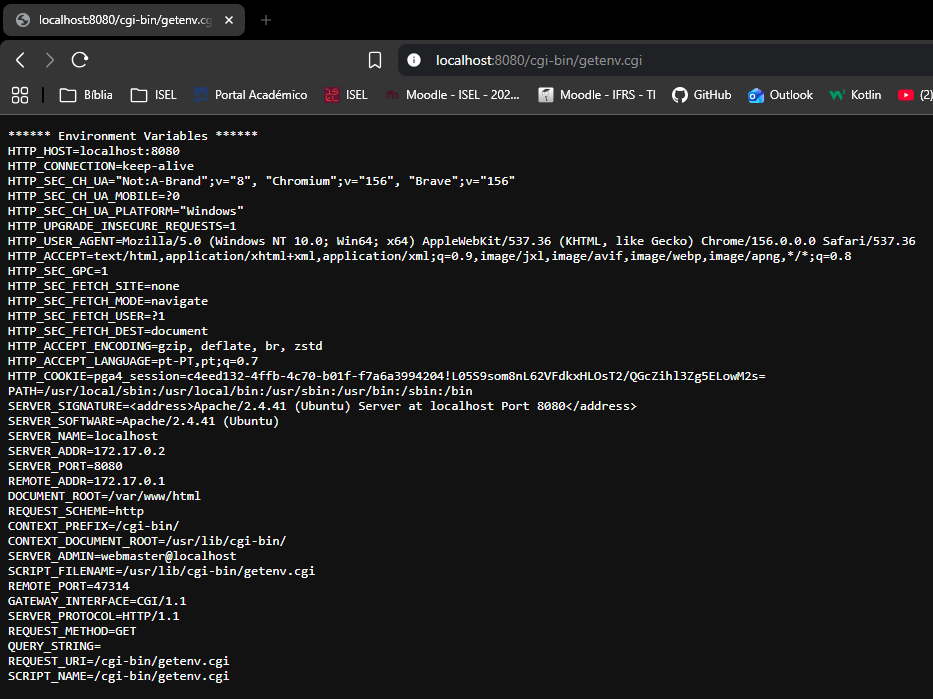
\includegraphics[width=0.85\textwidth]{02_preparacao/a_getenv-cgi.png}
\caption{Visualização no navegador --- endpoint \texttt{cgi-bin/getenv.cgi}}
\end{figure}

\begin{figure}[H]
\centering
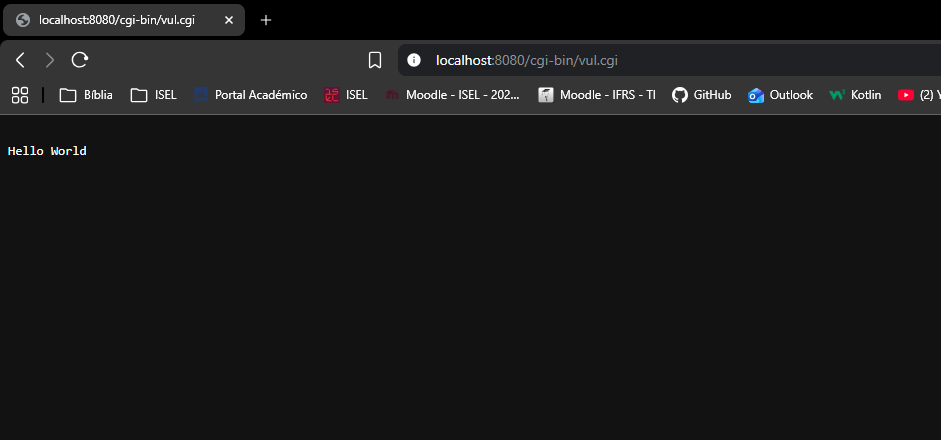
\includegraphics[width=0.85\textwidth]{02_preparacao/a_vul-cgi.png}
\caption{Visualização no navegador --- endpoint \texttt{cgi-bin/vul.cgi}}
\end{figure}

\paragraph{b) Análise do conteúdo dos CGI.}
Acedendo ao interior do contentor (\texttt{docker exec -it shellshock cat /usr/lib/cgi-bin/vul.cgi}),
regista-se o conteúdo de ambos os CGI.

\begin{figure}[H]
\centering
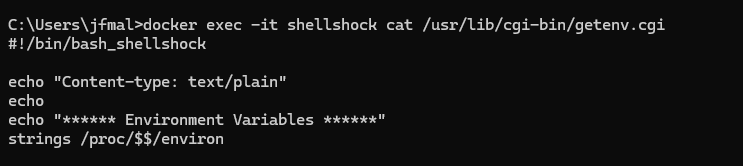
\includegraphics[width=0.85\textwidth]{02_preparacao/b_getenv-cgi.png}
\caption{Linha de comandos --- ficheiro \texttt{cgi-bin/getenv.cgi}}
\end{figure}

\begin{figure}[H]
\centering
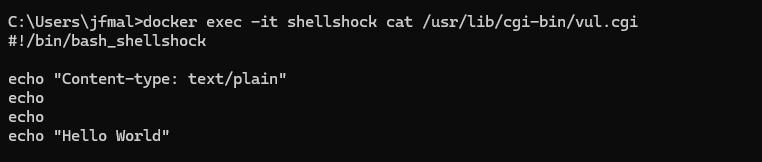
\includegraphics[width=0.85\textwidth]{02_preparacao/b_vul-cgi.png}
\caption{Linha de comandos --- ficheiro \texttt{cgi-bin/vul.cgi}}
\end{figure}

Quando é efetuado um pedido HTTP a um servidor Apache configurado para executar scripts CGI
(\textit{Common Gateway Interface}), o servidor processa o pedido e \textbf{converte
automaticamente os metadados e os cabeçalhos HTTP recebidos em variáveis de ambiente do
sistema operativo} antes de invocar o interpretador de comandos (Bash).

\begin{enumerate}
\item \textbf{Mapeamento de cabeçalhos HTTP:}
\begin{itemize}
\item Todos os cabeçalhos HTTP enviados pelo cliente (como \texttt{User-Agent},
\texttt{Host}, \texttt{Accept}, \texttt{Cookie}) são convertidos para maiúsculas e
guardados em variáveis de ambiente com o prefixo \texttt{HTTP\_}. Por exemplo, o cabeçalho
\texttt{User-Agent} passa a ser a variável \texttt{HTTP\_USER\_AGENT}.
\item Outras propriedades do pedido são mapeadas para variáveis específicas como
\texttt{REQUEST\_METHOD} (ex.: \texttt{GET}), \texttt{QUERY\_STRING},
\texttt{SERVER\_PROTOCOL} e \texttt{REMOTE\_ADDR}.
\end{itemize}

\item \textbf{Explicação do resultado do \texttt{getenv.cgi}:}
\begin{itemize}
\item O script emite primeiro os cabeçalhos HTTP exigidos pelo protocolo
(\texttt{Content-type: text/plain} seguido de uma linha em branco) e imprime o cabeçalho
descritivo \texttt{****** Environment Variables ******}.
\item De seguida, lê o pseudo-ficheiro virtual \texttt{/proc/\$\$/environ} mantido pelo
kernel do Linux, no qual \texttt{\$\$} representa o PID do próprio processo Bash em execução.
Este ficheiro armazena o bloco de memória com todas as variáveis de ambiente passadas ao
processo, separadas por bytes nulos.
\item O utilitário \texttt{strings} lê esse conteúdo em memória e extrai todas as sequências
de caracteres imprimíveis, exibindo cada variável de ambiente numa linha individual.
\end{itemize}
\end{enumerate}

Por essa razão, o resultado obtido é a \textbf{listagem de todas as variáveis de ambiente
criadas pelo Apache a partir do pedido HTTP do cliente} e lidas diretamente da memória do
processo no kernel, ilustrando como o servidor transmite dados não fiáveis do cliente para
o ambiente da \textit{shell}.

\subsection{Exploração (Red Team)}

\paragraph{a) Extração do ficheiro \texttt{/etc/passwd}.}
Através do endpoint \texttt{/cgi-bin/vul.cgi}, explora-se a vulnerabilidade Shellshock para
extrair o conteúdo de \texttt{/etc/passwd}. A exploração não depende do script que está no
\texttt{vul.cgi}, mas sim do facto de o CGI usar a shell Bash vulnerável; é ainda preciso
garantir que a resposta mantém conformidade com o protocolo HTTP.

\begin{figure}[H]
\centering
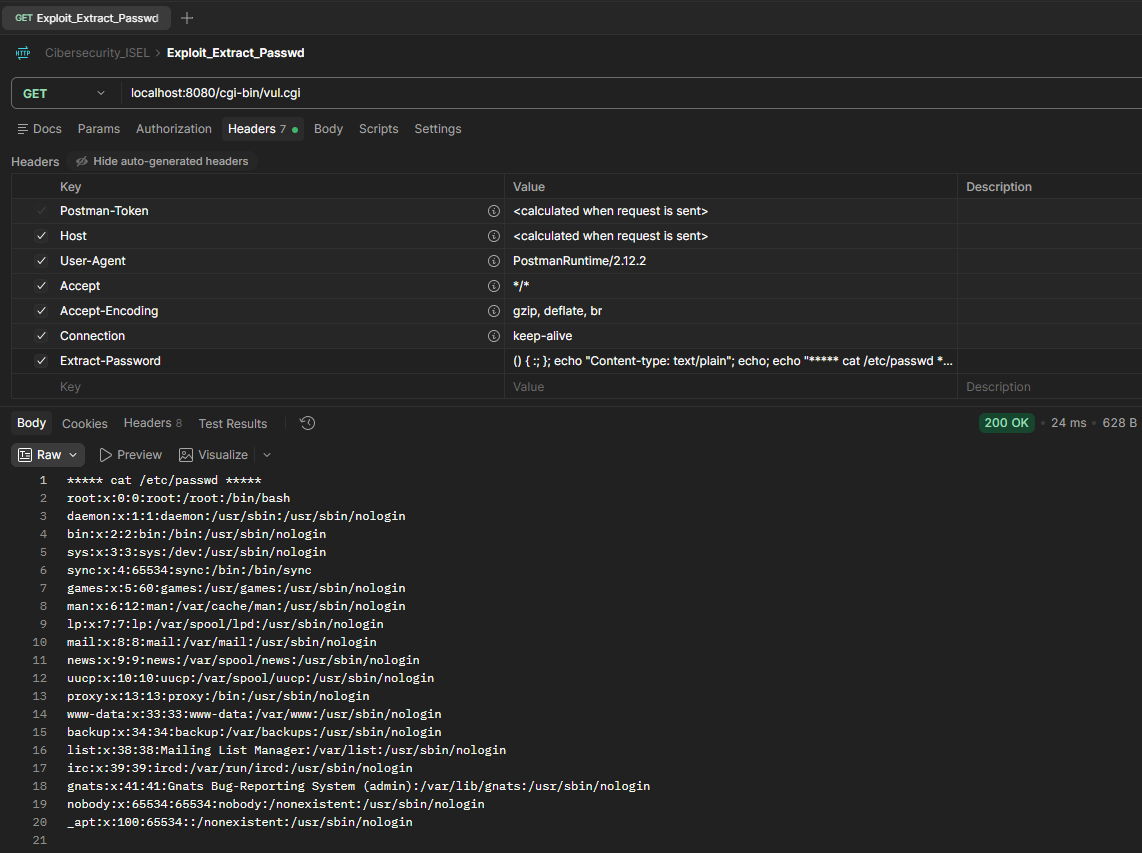
\includegraphics[width=0.85\textwidth]{03_exploracao/extract_passwd.png}
\caption{Postman --- extração do conteúdo de \texttt{/etc/passwd}}
\end{figure}

\begin{itemize}
\item \textbf{Header Name:} \texttt{Extract-Password}
\item \textbf{Header Value:} \texttt{() \{ :; \}; echo "Content-type: text/plain"; echo;
echo "***** cat /etc/passwd *****"; /bin/cat /etc/passwd;}
\end{itemize}

\textbf{Explicação do funcionamento:}
\begin{enumerate}
\item \textbf{Mapeamento do Apache:} ao receber o pedido com o cabeçalho personalizado
\texttt{Extract-Password}, o Apache converte o seu nome e valor para a variável de ambiente
\texttt{HTTP\_EXTRACT\_PASSWORD}.
\item \textbf{Invocação do CGI:} o Apache chama o script \texttt{/cgi-bin/vul.cgi}, que invoca
o interpretador \texttt{/bin/bash} vulnerável.
\item \textbf{Exploração da falha (CVE-2014-6271):} o Bash lê as variáveis de ambiente
importadas. Ao detetar que a variável começa pela assinatura de função \texttt{() \{ :; \};},
sofre um erro de \textit{parsing} e \textbf{executa incondicionalmente os comandos anexados
a seguir à declaração}.
\item \textbf{Conformidade HTTP:} a instrução \texttt{echo "Content-type: text/plain"; echo;}
envia os cabeçalhos necessários seguidos de uma linha em branco, impedindo que o Apache
devolva um erro \texttt{500 Internal Server Error}.
\item \textbf{Resultado:} o comando \texttt{/bin/cat /etc/passwd} é executado no servidor e o
conteúdo das contas do sistema é impresso no corpo da resposta.
\end{enumerate}

\paragraph{b) Criação de ficheiro de evidência em \texttt{/tmp}.}
Criação do ficheiro \texttt{evidence\_<numero\_aluno>.txt} contendo a data atual e o nome.

\begin{figure}[H]
\centering
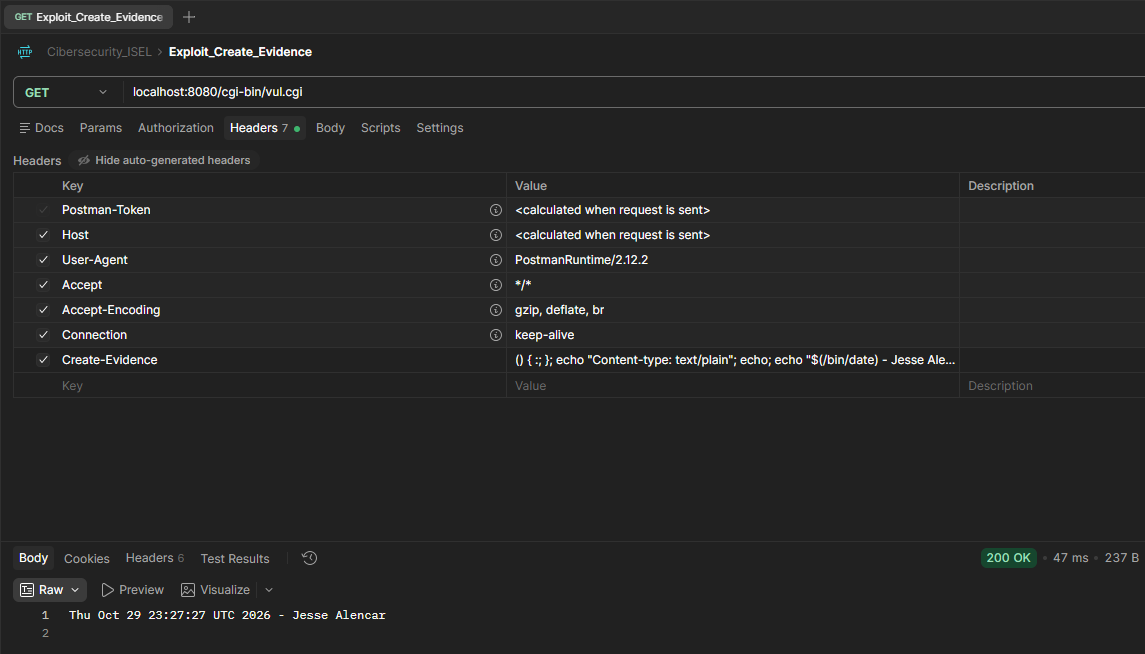
\includegraphics[width=0.85\textwidth]{03_exploracao/create_evidence.png}
\caption{Postman --- criação do ficheiro de evidência}
\end{figure}

\begin{itemize}
\item \textbf{Header Name:} \texttt{Create-Evidence}
\item \textbf{Header Value:} \texttt{() \{ :; \}; echo "Content-type: text/plain"; echo;
echo "\$(/bin/date) - Jesse Alencar" > /tmp/evidence\_51745.txt;
/bin/cat /tmp/evidence\_51745.txt;}
\item \textbf{Resultado:} o comando executa \texttt{/bin/date}, concatena com o nome e
redireciona a saída para \texttt{/tmp/evidence\_51745.txt}. De seguida, faz \texttt{cat} do
ficheiro recém-criado, confirmando a escrita imediata.
\end{itemize}

\begin{figure}[H]
\centering
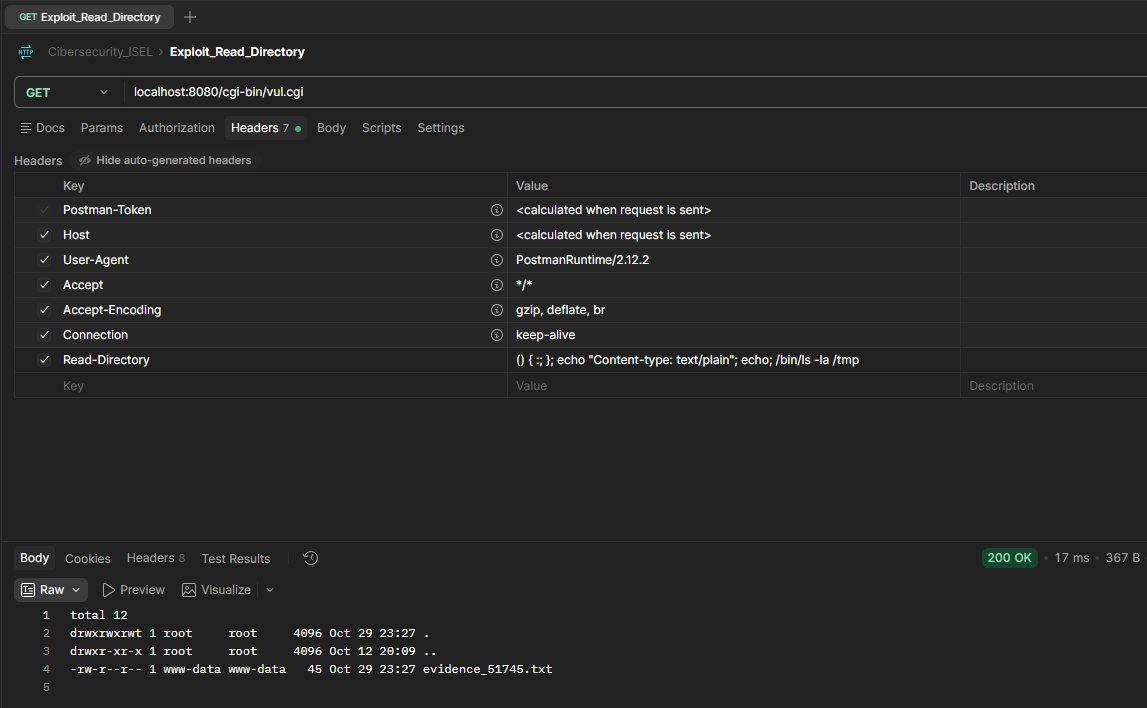
\includegraphics[width=0.85\textwidth]{03_exploracao/read_directory.png}
\caption{Postman --- leitura da diretoria \texttt{/tmp}}
\end{figure}

\begin{itemize}
\item \textbf{Header Name:} \texttt{Read-Evidence}
\item \textbf{Header Value:} \texttt{() \{ :; \}; echo "Content-type: text/plain"; echo;
/bin/ls -la /tmp}
\item \textbf{Resultado:} \texttt{/bin/ls -la /tmp} devolve a listagem detalhada do diretório,
comprovando a existência, o tamanho, as permissões e o proprietário do ficheiro
\texttt{evidence\_51745.txt}.
\end{itemize}

\paragraph{c) Query string como vetor de ataque.}
Os pedidos HTTP GET podem enviar dados no URL após a marca \texttt{?}, na \textit{query
string}. Demonstra-se que esta aparece numa variável de ambiente e avalia-se se pode lançar
o ataque.

\begin{figure}[H]
\centering
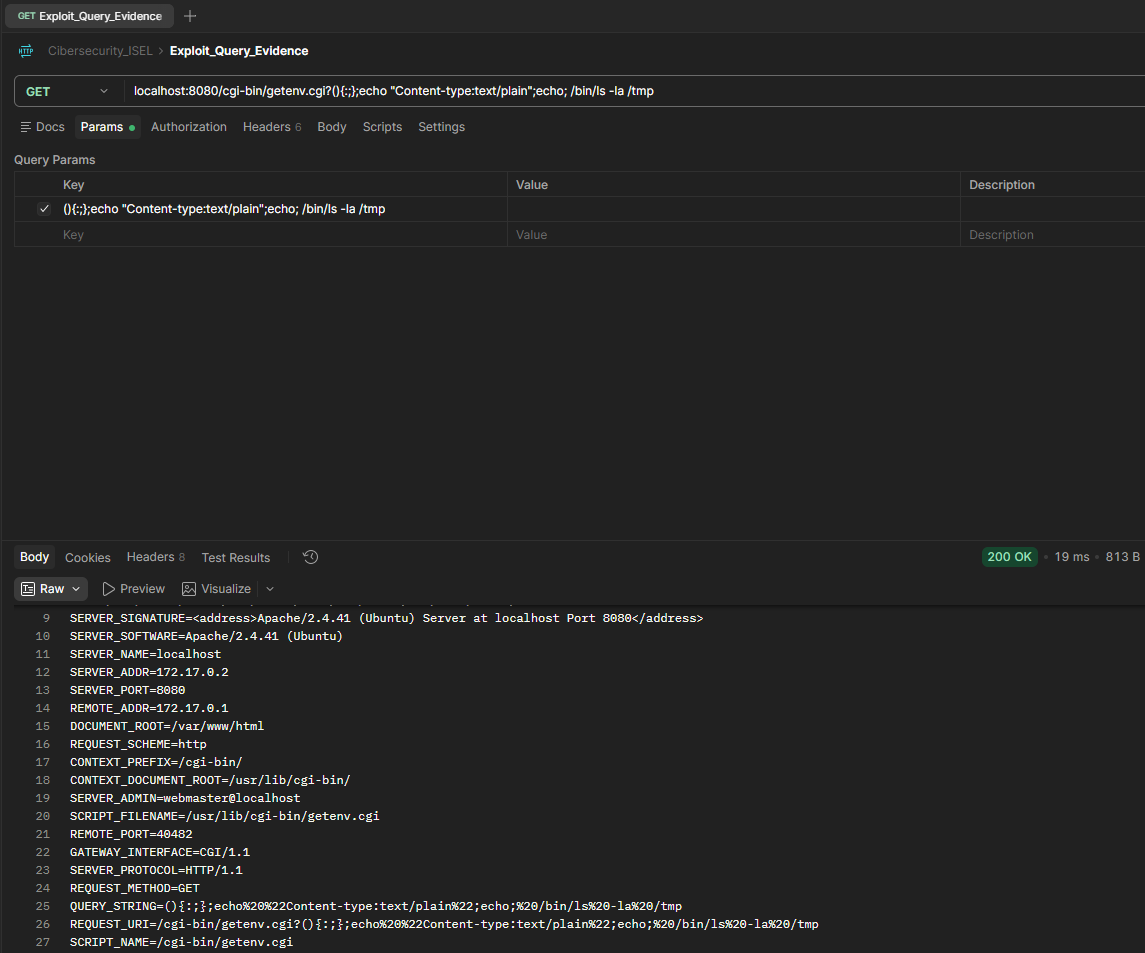
\includegraphics[width=0.85\textwidth]{03_exploracao/test_query_read.png}
\caption{Postman --- teste da query string como meio de exploração}
\end{figure}

\begin{itemize}
\item \textbf{Aparecimento na variável de ambiente:} quando um GET inclui dados a seguir ao
\texttt{?}, o Apache guarda esse valor na variável \texttt{QUERY\_STRING}, o que é confirmado
ao chamar o \texttt{getenv.cgi}.
\item \textbf{Viabilidade:} teoricamente, se o valor da \texttt{QUERY\_STRING} começasse
exatamente por \texttt{() \{ :; \};}, o Bash executaria os comandos. Na prática, porém:
\begin{enumerate}
\item No formato padrão \texttt{?param=() \{ :; \};}, a variável fica
\texttt{QUERY\_STRING=param=() \{ :; \};}; como não começa por \texttt{() \{}, o bug não é
ativado.
\item Clientes e servidores aplicam \textit{percent-encoding}, convertendo \texttt{\{\}} em
\texttt{\%7B\%7D}, o que impede o Bash de reconhecer o padrão de função.
\end{enumerate}
\item \textbf{Conclusão:} os cabeçalhos HTTP personalizados são um vetor muito mais eficaz,
pois o Apache injeta os seus valores intactos nas variáveis \texttt{HTTP\_*} sem adicionar
nomes de parâmetros nem aplicar \textit{percent-encoding}.
\end{itemize}

\subsection{Análise de permissões}

\paragraph{a) Acesso a \texttt{/etc/shadow}.}

\begin{figure}[H]
\centering
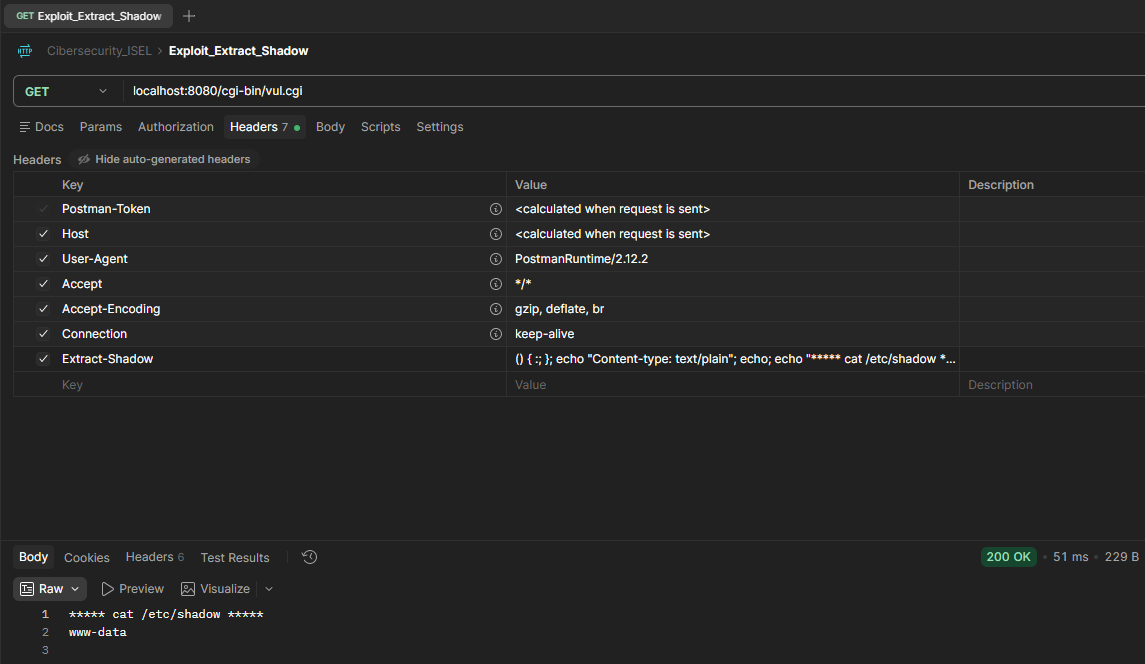
\includegraphics[width=0.85\textwidth]{03_exploracao/extract_shadow.png}
\caption{Postman --- tentativa de extração de \texttt{/etc/shadow}}
\end{figure}

\begin{itemize}
\item \textbf{Header Name:} \texttt{Extract-Shadow}
\item \textbf{Header Value:} \texttt{() \{ :; \}; echo "Content-type: text/plain"; echo;
echo "***** cat /etc/shadow *****"; echo "\$(/bin/whoami)"; /bin/cat /etc/shadow;}
\item \textbf{Resultado:} o comando imprime o utilizador ativo (\texttt{www-data}), mas falha
a leitura com a mensagem \texttt{cat: /etc/shadow: Permission denied}.
\item \textbf{Explicação:} por aplicação do princípio do menor privilégio, o Apache e os seus
processos CGI filhos correm sob a conta sem privilégios \texttt{www-data}. Como
\texttt{/etc/shadow} tem permissões de leitura restritas ao superutilizador \texttt{root}, o
sistema operativo nega o acesso.
\end{itemize}

\newpage
% ==================================================================
\section{Parte 2 --- Análise estática com CodeQL (WebGoat / Juice Shop)}
% ==================================================================

\subsection{A.5.b --- Deteção de credenciais embutidas (HardcodedCredentials)}

\paragraph{i) \texttt{@precision}.}
O valor é \texttt{@precision low}. Indica que a query tem uma taxa elevada de falsos
positivos, ou seja, muitos dos alertas podem não ser problemas reais. Por isso, estas queries
não vêm na \textit{suite} padrão do \textit{code scanning} e os resultados precisam de revisão
manual. Os valores possíveis são \texttt{low}, \texttt{medium}, \texttt{high} e
\texttt{very-high}.

\paragraph{ii) Como decide que um campo contém uma password.}
A decisão baseia-se apenas no \textbf{nome da variável}. A query usa a classe
\texttt{PasswordVariable}, definida em \texttt{HardcodedCredentials.qll:69}:

\begin{lstlisting}
this.getName().regexpMatch("(?i)(encrypted|old|new)?pass(wd|word|code|phrase)(chars|value)?")
\end{lstlisting}

Ou seja, uma variável conta como password se o nome inteiro (sem distinguir maiúsculas de
minúsculas) for algo como \texttt{password}, \texttt{passwd}, \texttt{passcode},
\texttt{newPassword}, \texttt{passwordValue}, etc. Depois, o predicado
\texttt{passwordFieldAssignedHardcodedValue} (em \texttt{HardcodedPasswordField.ql}) exige três
condições:
\begin{enumerate}
\item a variável é um \textbf{campo} da classe (\texttt{f instanceof Field});
\item é-lhe atribuída uma \textbf{constante de compilação} (\texttt{CompileTimeConstantExpr}),
por exemplo um literal;
\item essa constante \textbf{não é a string vazia} \texttt{""}.
\end{enumerate}

\paragraph{iii) É análise de fluxo de dados?}
Não. É uma análise \textbf{sintática/estrutural} sobre a AST: verifica o nome do campo e se o
valor atribuído diretamente é uma constante. Não importa \texttt{DataFlow} nem
\texttt{TaintTracking}, nem segue o valor para onde é usado. Se a password passasse por outra
variável ou por um método antes de chegar ao campo, a query já não a detetava.

\paragraph{c) Execução da query.}
A interrogação \texttt{HardcodedPasswordField.ql} foi executada sobre a base de dados
\texttt{webgoat-database}, produzindo 2 resultados: um campo com valor embutido em
\texttt{SolutionConstants.java:10} e outro em \texttt{JWTRefreshEndpoint.java:45}.

\begin{figure}[H]
\centering
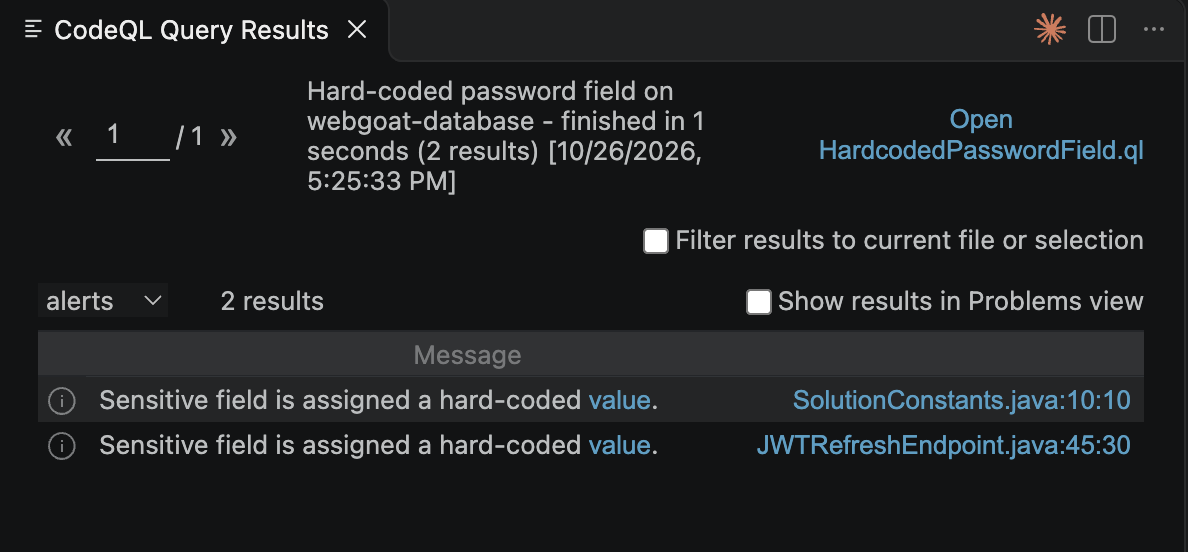
\includegraphics[width=0.9\textwidth]{5.c.png}
\caption{Resultados da query \texttt{HardcodedPasswordField.ql} (2 campos de password detetados)}
\end{figure}

\subsection{A.5.d --- JWT e falso negativo}

\paragraph{i) Estrutura JWT e operação criptográfica.}
Um JWT tem três partes codificadas em Base64URL e separadas por pontos:
\texttt{header.payload.signature}.
\begin{itemize}
\item \textbf{Header:} JSON com o tipo e o algoritmo, por exemplo
\texttt{\{"alg":"HS512","typ":"JWT"\}}.
\item \textbf{Payload:} as \textit{claims}, isto é, os dados sobre o utilizador. Aqui são
\texttt{\{"admin":"false","user":"Jerry"\}} mais o \texttt{iat}. Só está codificado, não cifrado,
por isso qualquer pessoa o consegue ler.
\item \textbf{Signature:} \texttt{HMAC-SHA512(base64url(header) + "." + base64url(payload),
segredo)}.
\end{itemize}
A operação que depende do segredo é o \textbf{HMAC (HS512)}, uma assinatura simétrica. A mesma
chave serve para \textbf{gerar} a assinatura ao emitir o token e para a \textbf{verificar}
quando o token volta ao servidor. Garante a \textbf{integridade e autenticidade} do token, mas
não a confidencialidade.

\paragraph{ii) Porque é que a query não o detetou.}
A classe \texttt{PasswordVariable} só aceita nomes que correspondam \textbf{na totalidade} a:
\begin{lstlisting}
(?i)(encrypted|old|new)?pass(wd|word|code|phrase)(chars|value)?
\end{lstlisting}
Em CodeQL, o \texttt{regexpMatch} está implicitamente ancorado: tem de corresponder ao nome
todo, não apenas a uma parte. O único prefixo permitido é \texttt{encrypted}, \texttt{old} ou
\texttt{new}. Como \texttt{JWT\_PASSWORD} começa por \texttt{JWT\_}, que não está nessa lista, a
correspondência falha e o campo nunca é considerado um \texttt{PasswordVariable}. O campo
\texttt{PASSWORD} da linha 45 corresponde exatamente, porque a regex ignora maiúsculas e
minúsculas e não tem prefixo. Há ainda uma limitação mais geral: a query baseia-se apenas em
nomes --- uma chave guardada numa variável chamada \texttt{secret}, \texttt{key} ou
\texttt{signingKey} também nunca seria detetada.

\paragraph{iii) Classificação.}
É um \textbf{falso negativo}. Existe de facto uma vulnerabilidade (um segredo criptográfico
embutido no código), mas a ferramenta \textbf{não a reportou}.

\subsection{A.5.e --- Impacto do segredo JWT comprometido}

Com o \texttt{JWT\_PASSWORD}, o atacante consegue \textbf{forjar tokens válidos com quaisquer
claims}, sem precisar de credenciais nem de fazer login:
\begin{itemize}
\item \textbf{Escalar privilégios:} gerar um token com \texttt{"admin": "true"} e aceder a
funções de administração.
\item \textbf{Fazer-se passar por qualquer utilizador:} pôr \texttt{"user": "Tom"} ou outro
nome qualquer e agir em nome dessa pessoa. Não está limitado ao Jerry.
\item \textbf{Persistência:} criar tokens sem expiração, ou com \texttt{iat}/\texttt{exp}
manipulados. Continuam válidos mesmo que as passwords dos utilizadores mudem, até o segredo ser
rodado.
\item \textbf{Contornar a autenticação por completo:} o endpoint de login deixa de ter
qualquer importância.
\end{itemize}

\subsection{A.5.f --- Path Traversal (CWE-22)}

Foi utilizada a interrogação \texttt{Security/CWE/CWE-022/TaintedPath.ql}, que usa análise de
fluxo de dados para encontrar dados controlados pelo utilizador usados na construção de
caminhos de ficheiros.

\textbf{Resultado em \texttt{ProfileUploadBase.java}:} linha 52, \textit{"This path depends on a
user-provided value."}

\begin{center}
\begin{tabularx}{\textwidth}{@{}C{0.6cm} l L@{}}
\toprule
\textbf{\#} & \textbf{Localização} & \textbf{Descrição} \\
\midrule
1 & \texttt{ProfileUpload.java:41} & \textbf{Source:} parâmetro \texttt{fullName} do pedido HTTP \\
2 & \texttt{ProfileUpload.java:43} & \texttt{fullName} é passado ao método \texttt{execute()} \\
3 & \texttt{ProfileUploadBase.java:40} & \texttt{fullName} chega ao método \texttt{execute()} \\
4 & \texttt{ProfileUploadBase.java:52} & \textbf{Sink:} criação do ficheiro com \texttt{createNewFile()} \\
\bottomrule
\end{tabularx}
\end{center}

\begin{lstlisting}[language=Java]
var uploadedFile = new File(uploadDirectory, fullName);
uploadedFile.createNewFile();
FileCopyUtils.copy(file.getBytes(), uploadedFile);
\end{lstlisting}

\begin{figure}[H]
\centering
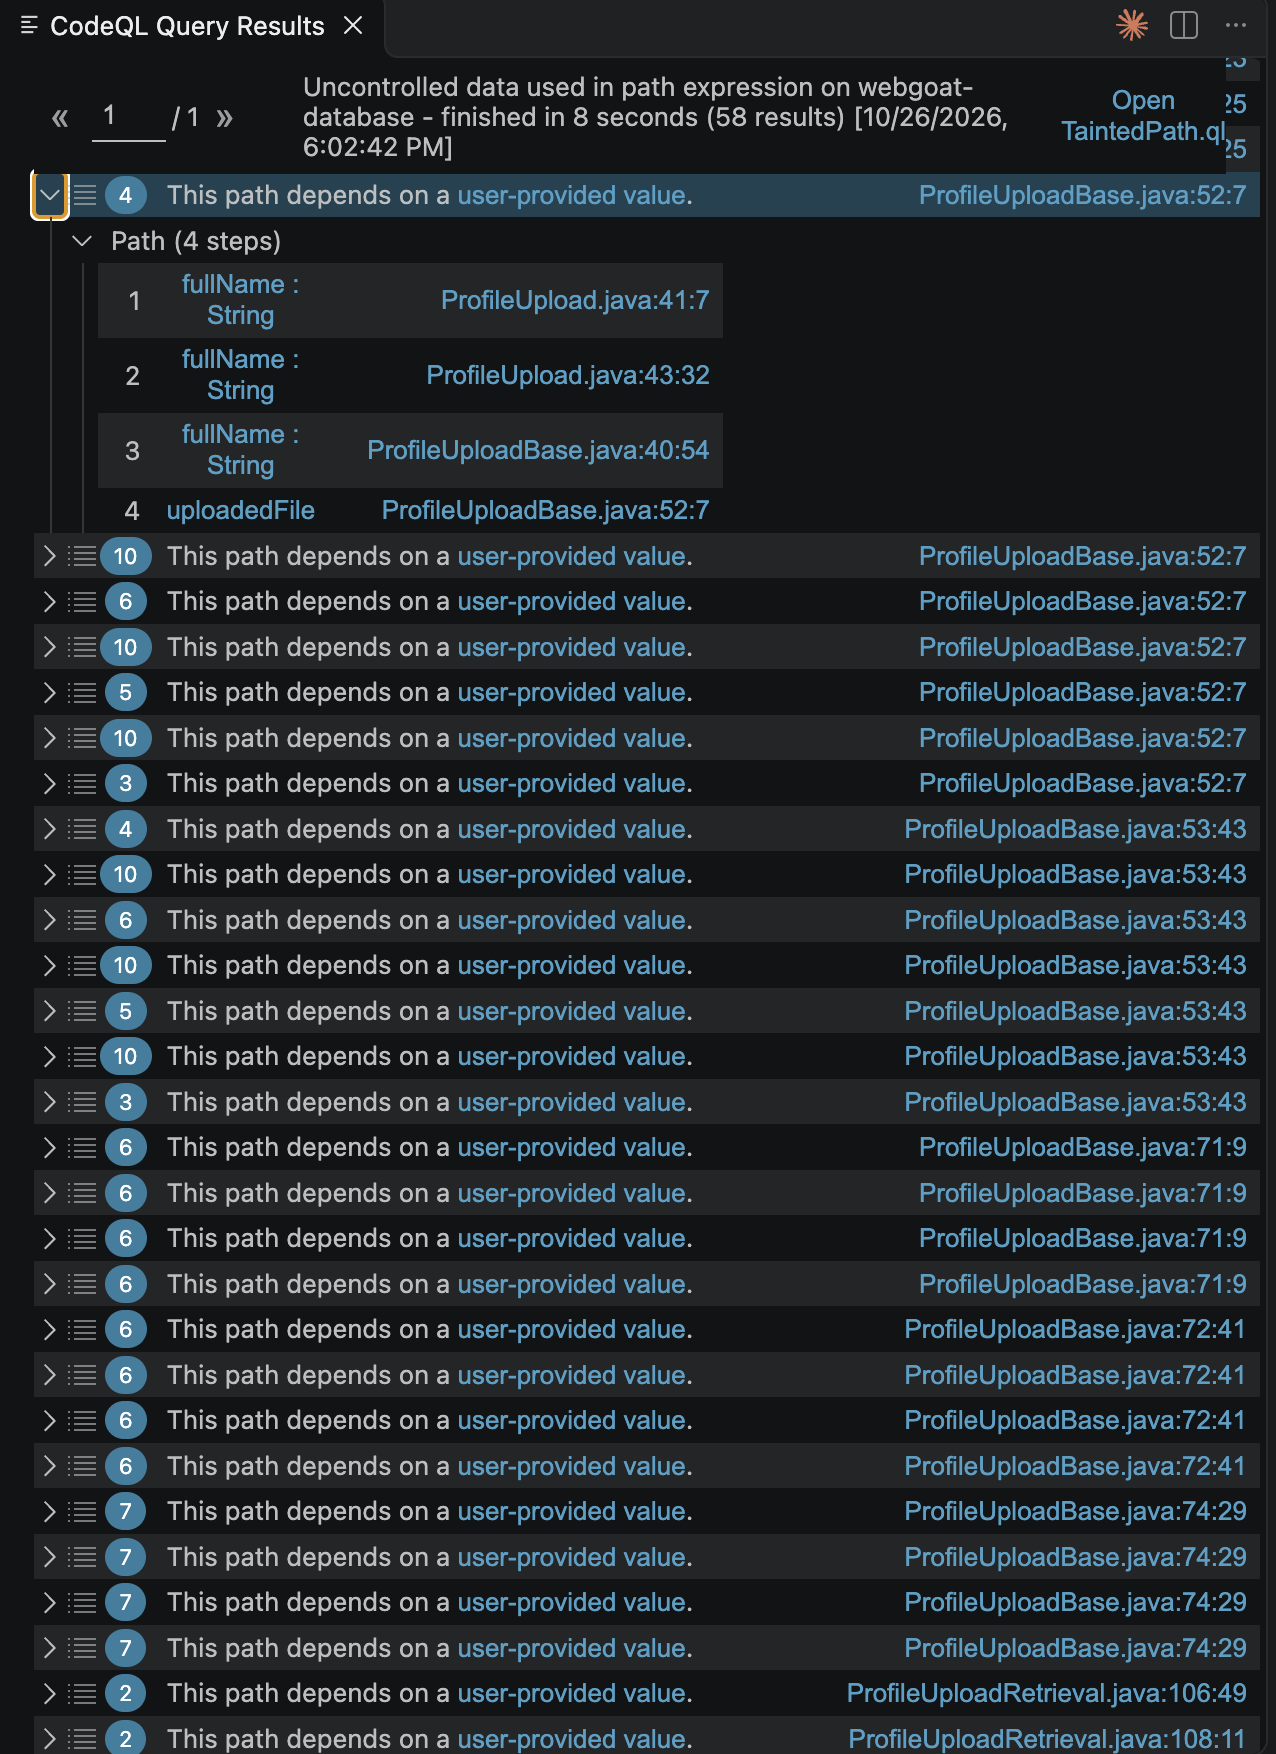
\includegraphics[height=0.75\textheight]{5f.png}
\caption{Resultados do \texttt{TaintedPath.ql} --- caminho de 4 passos de \texttt{fullName}
até \texttt{ProfileUploadBase.java:52}}
\end{figure}

\textbf{Vetor de ataque:} o endpoint \texttt{POST /PathTraversal/profile-upload} serve para
carregar a fotografia de perfil, que devia ser guardada em
\texttt{.../PathTraversal/<username>/<fullName>}. Como o valor de \texttt{fullName} é enviado
pelo utilizador e não é validado, um atacante pode intercetar o pedido e colocar sequências
\texttt{../} nesse campo, por exemplo \texttt{fullName = ../../../tmp/malicioso}. Cada
\texttt{../} sobe um nível na árvore de diretórios, pelo que o ficheiro é escrito \textbf{fora
da pasta prevista}. Como o atacante controla o caminho e o conteúdo do ficheiro, pode criar ou
sobrescrever ficheiros em qualquer pasta onde a aplicação tenha permissão de escrita (ficheiros
de configuração ou de outros utilizadores). Em certos cenários pode chegar a executar código no
servidor, por exemplo colocando um script num diretório servido pela aplicação.

\subsection{A.5.g --- Correção e reanálise}

A base de dados foi regenerada
(\texttt{codeql database create webgoat-database --language=java --build-mode=none --overwrite})
e a interrogação \texttt{TaintedPath.ql} foi novamente executada.

\textbf{Resultado:} o CodeQL \textbf{deixou de assinalar} a vulnerabilidade no método
\texttt{execute()}. Os alertas anteriormente reportados em \texttt{createNewFile()} e
\texttt{FileCopyUtils.copy()} deixaram de aparecer para todos os endpoints que invocam este
método.

\textbf{Justificação:} \texttt{getCanonicalPath()} devolve o caminho absoluto normalizado, com
as sequências \texttt{../} e os links simbólicos resolvidos. A comparação com
\texttt{startsWith(uploadDirectory.getCanonicalPath() + File.separator)} garante que o ficheiro
final fica dentro do diretório de upload. A inclusão de \texttt{File.separator} evita que um
diretório como \texttt{.../rodrigo-evil} seja aceite como prefixo de \texttt{.../rodrigo}. As
bibliotecas do CodeQL reconhecem este padrão como \textit{sanitizer guard} de path traversal,
pelo que o fluxo de dados contaminados é interrompido antes de chegar aos \textit{sinks}.

Os resultados que permanecem (\texttt{cleanupAndCreateDirectoryForUser()}, linhas 78, 79 e 81)
já existiam antes da alteração e têm como \textit{source} o \texttt{username}. Esse valor é
obtido da sessão autenticada (\texttt{@CurrentUsername} $\rightarrow$
\texttt{@AuthenticationPrincipal}) e não do pedido HTTP, e está restrito ao padrão
\texttt{[a-z0-9-]*}. Tratam-se de falsos positivos não relacionados com o método
\texttt{execute()}.

\begin{figure}[H]
\centering
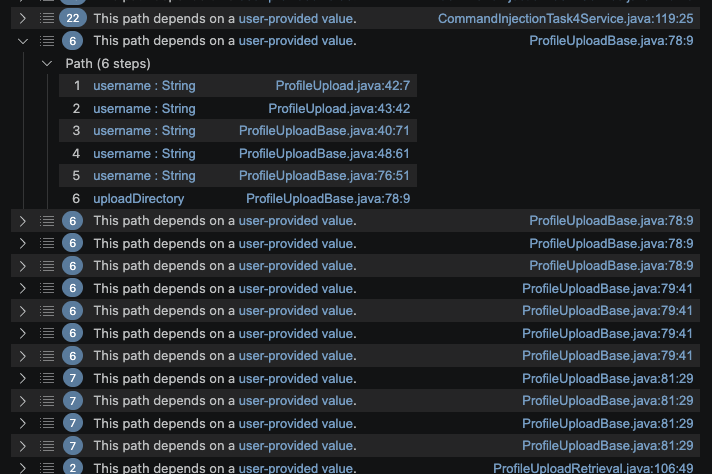
\includegraphics[width=0.85\textwidth]{5g.png}
\caption{Após a correção, os alertas em \texttt{execute()} desaparecem; permanecem apenas os
resultados com \textit{source} \texttt{username} em \texttt{cleanupAndCreateDirectoryForUser()}}
\end{figure}

\subsection{A.5.h --- Classificação OWASP}

\textbf{OWASP Top 10:2025:} a vulnerabilidade insere-se na categoria \textbf{A01:2025 --- Broken
Access Control}. A CWE-22 (\textit{Improper Limitation of a Pathname to a Restricted Directory ---
'Path Traversal'}) faz parte da lista de CWEs mapeadas para esta categoria: a falha permite ao
atacante aceder a recursos do sistema de ficheiros (neste caso, escrever neles) fora do diretório
a que deveria estar restrito, contornando as restrições de acesso pretendidas pela aplicação.

\textbf{OWASP ASVS 5.0 --- V5.3 File Storage:} o código viola o requisito \textbf{5.3.2 (Nível
1)}, que exige que, ao construir caminhos para operações sobre ficheiros, a aplicação utilize
dados gerados internamente ou confiáveis em vez de nomes de ficheiro submetidos pelo utilizador.
Se for necessário usar nomes ou metadados fornecidos pelo utilizador, estes devem ser sujeitos a
validação e sanitização estritas, de forma a prevenir \textit{path traversal}, inclusão de
ficheiros locais ou remotos (LFI/RFI) e SSRF. No método \texttt{execute()} original, o parâmetro
\texttt{fullName} é usado diretamente em \texttt{new File(uploadDirectory, fullName)} sem
qualquer validação. A correção aplicada em A.5.g passa a cumprir este requisito. O requisito
relacionado \textbf{5.3.1 (Nível 1)} exige que ficheiros carregados para pastas públicas não
sejam executados como código no servidor; o seu cumprimento mitigaria a consequência mais grave
do ataque (execução de uma \textit{webshell}).

\subsection{C.1 --- Workflow CodeQL}

Fork do grupo: \url{https://github.com/RodrigoVitorino/juice-shop}

O \textit{trigger} do workflow "CodeQL Scan" foi alterado para \texttt{workflow\_dispatch}, de
forma a permitir a sua execução manual.

\begin{figure}[H]
\centering
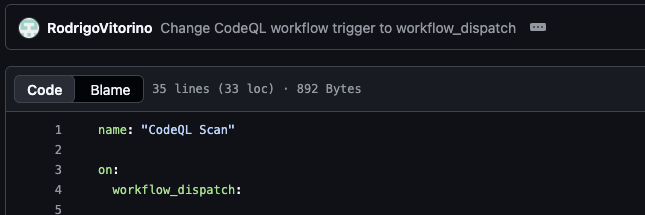
\includegraphics[width=0.75\textwidth]{C1.png}
\caption{Workflow "CodeQL Scan" configurado com o \textit{trigger} \texttt{workflow\_dispatch}}
\end{figure}

\subsection{C.2 --- Execução manual e inicialização da base de dados}

O workflow "CodeQL Scan" foi executado manualmente em \textbf{Actions $\rightarrow$ CodeQL Scan
$\rightarrow$ Run workflow} (evento \texttt{workflow\_dispatch}) e terminou com sucesso.

\textbf{Etapa:} a base de dados é inicializada na etapa \textbf{Initialize CodeQL}, que
corresponde à ação \texttt{github/codeql-action/init@v3}.

\textbf{Comando} (extraído dos logs):
\begin{lstlisting}
/opt/hostedtoolcache/CodeQL/2.27.3/x64/codeql/codeql database init \
  --force-overwrite \
  --db-cluster /home/runner/work/_temp/codeql_databases \
  --source-root=/home/runner/work/juice-shop/juice-shop \
  --calculate-language-specific-baseline \
  --sublanguage-file-coverage \
  --extractor-include-aliases \
  --language=javascript \
  --codescanning-config=/home/runner/work/_temp/user-config.yaml
\end{lstlisting}

O comando \texttt{codeql database init} cria a estrutura da base de dados para a linguagem
\texttt{javascript} (que inclui TypeScript) a partir do código-fonte em \texttt{--source-root},
usando a configuração definida no workflow. A extração do código e a finalização da base de dados
acontecem nas etapas seguintes (\textit{Autobuild} e \textit{Perform CodeQL Analysis}), seguidas
da execução das queries.

\textbf{Localização da base de dados:} a opção \texttt{--db-cluster} indica que as bases de dados
são criadas em \texttt{/home/runner/work/\_temp/codeql\_databases/}, numa subpasta por linguagem.
Este diretório pertence ao \textit{runner} (a máquina virtual temporária do GitHub Actions), que
é destruída no fim do job --- a base de dados não fica no repositório. O que persiste são os
resultados da análise, em formato SARIF, consultáveis em \textbf{Security $\rightarrow$ Code
scanning}.

\subsection{C.3 --- SQL Injection (CWE-89) em \texttt{routes/search.ts}}

\textbf{Alerta:} \textit{Database query built from user-controlled sources} (\#13), regra CodeQL
\texttt{js/sql-injection}, severidade \textbf{High}, CWEs associadas: CWE-89, CWE-90, CWE-943.

\begin{lstlisting}
21  let criteria: any = req.query.q === 'undefined' ? '' : req.query.q ?? ''
22  criteria = (criteria.length <= 200) ? criteria : criteria.substring(0, 200)
23  models.sequelize.query(`SELECT * FROM Products WHERE ((name LIKE '%${criteria}%'
        OR description LIKE '%${criteria}%') AND deletedAt IS NULL) ORDER BY name`)
\end{lstlisting}

\paragraph{Source e sink.}
O CodeQL reporta um caminho de fluxo de dados com 6 passos, todos em \texttt{routes/search.ts}:

\begin{center}
\begin{tabularx}{\textwidth}{@{}l C{0.9cm} l L@{}}
\toprule
\textbf{Passo} & \textbf{Linha} & \textbf{Nó} & \textbf{Descrição} \\
\midrule
1 -- Source & 21 & \texttt{req.query.q} & Parâmetro \texttt{q} da query string (\texttt{GET /rest/products/search?q=...}), controlado pelo utilizador \\
2 & 21 & \texttt{criteria} & O valor é atribuído à variável \texttt{criteria} \\
3 & 22 & \texttt{criteria} & Se o comprimento $\leq$ 200, o ternário devolve o valor inalterado \\
4 & 22 & \texttt{criteria = ...} & O resultado é atribuído de novo a \texttt{criteria} \\
5 & 23 & \texttt{\$\{criteria\}} & O valor é interpolado na \textit{template string} da consulta \\
6 -- Sink & 23 & \texttt{sequelize.query} & A string SQL é passada a \texttt{models.sequelize.query(...)} e executada \\
\bottomrule
\end{tabularx}
\end{center}

O caminho completo reportado pelo GitHub Code scanning (6 passos em \texttt{routes/search.ts}) é
apresentado nas figuras seguintes.

\begin{figure}[H]
\centering
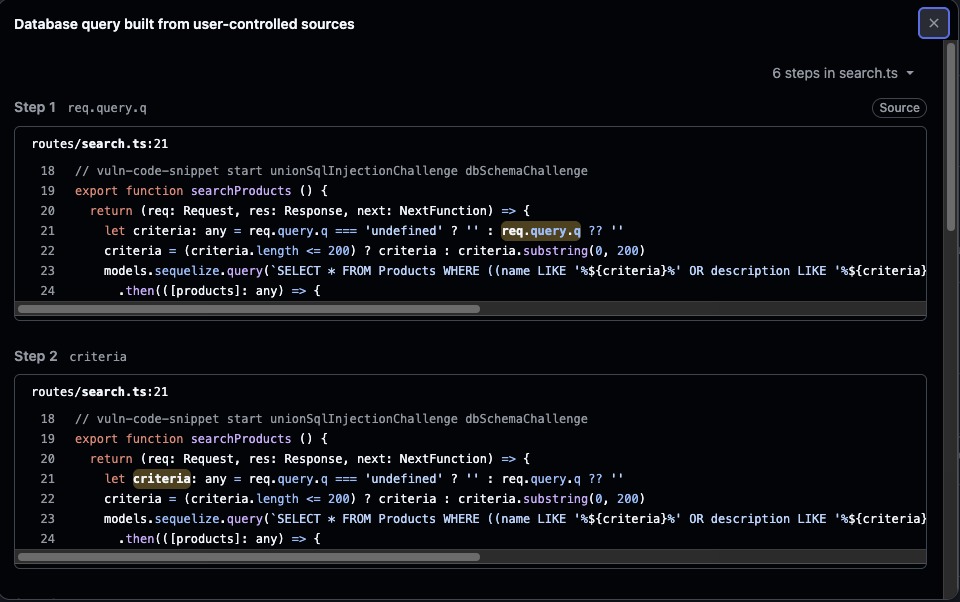
\includegraphics[width=0.85\textwidth]{C3_parte1.png}
\caption{Caminho de fluxo de dados do SQL injection --- passos 1 e 2 (\textit{source})}
\end{figure}

\begin{figure}[H]
\centering
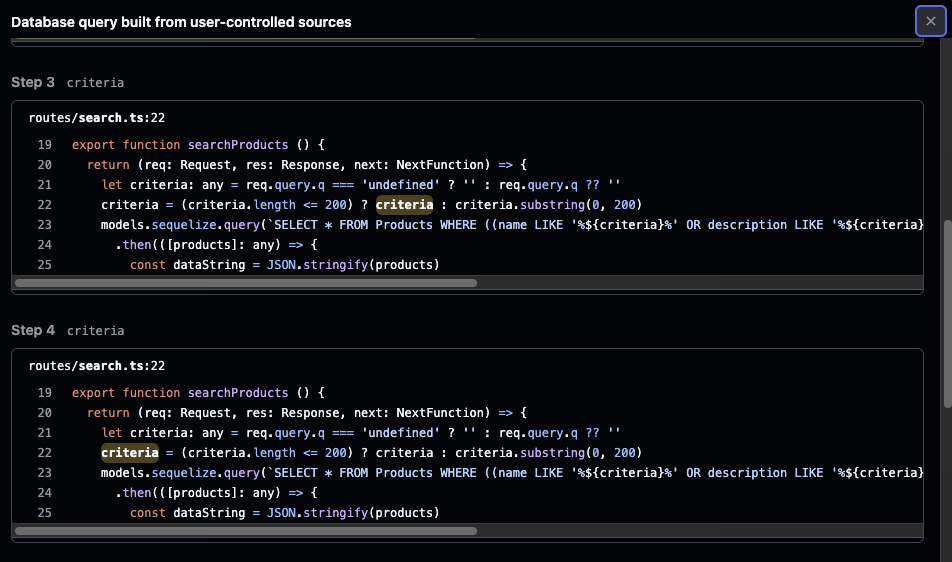
\includegraphics[width=0.85\textwidth]{C3_parte2.png}
\caption{Caminho de fluxo de dados do SQL injection --- passos 3 e 4}
\end{figure}

\begin{figure}[H]
\centering
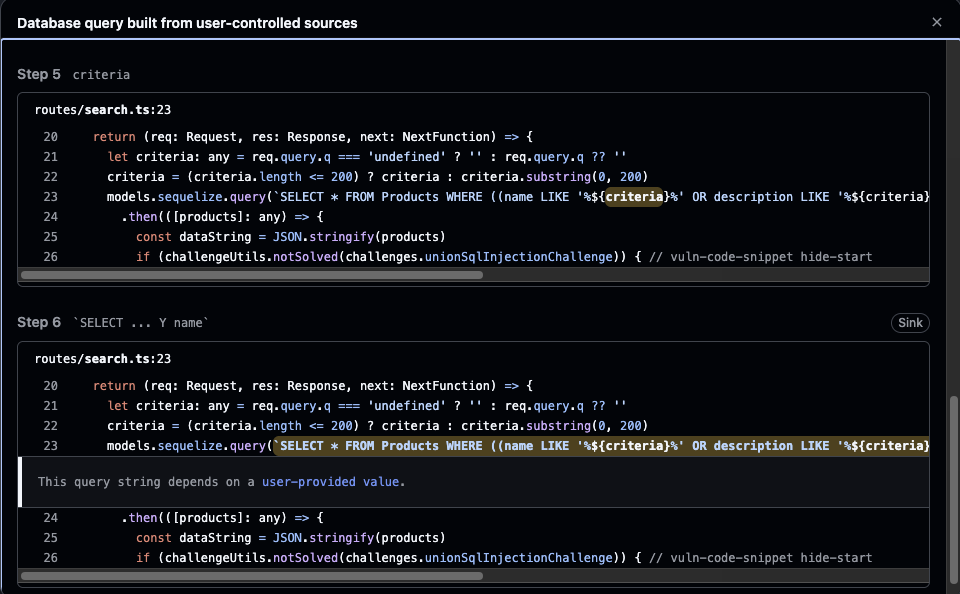
\includegraphics[width=0.85\textwidth]{C3_parte3.png}
\caption{Caminho de fluxo de dados do SQL injection --- passos 5 e 6 (\textit{sink})}
\end{figure}

Ao longo do caminho, o valor não passa por nenhuma operação de neutralização de caracteres
especiais. A única transformação possível, \texttt{substring(0, 200)}, limita apenas o
comprimento e nem sequer é aplicada no caminho reportado (passo 3), pelo que o valor original do
utilizador chega intacto à instrução SQL.

\paragraph{Justificação.}
O CodeQL usa análise de fluxo de dados (\textit{taint tracking}) e identifica que um valor
proveniente de uma \textit{source} remota (\texttt{req.query}) chega, sem passar por nenhum
sanitizador reconhecido, a um \textit{sink} que executa SQL (\texttt{sequelize.query}). O input
do utilizador é concatenado no texto da instrução SQL em vez de ser passado como parâmetro.
Assim, caracteres como \texttt{'} e \texttt{)} alteram a estrutura da instrução, e não apenas os
dados, o que corresponde à definição da CWE-89.

\textbf{Exemplo de exploração:}
\begin{lstlisting}
GET /rest/products/search?q=xyz')) UNION SELECT id, email, password, '4','5','6','7','8','9' FROM Users--
\end{lstlisting}
A instrução passa a devolver, juntamente com os produtos, os emails e os \textit{hashes} de
password de todos os utilizadores. O \texttt{--} comenta o resto da instrução original. Também é
possível extrair o esquema da base de dados (por exemplo, a partir de \texttt{sqlite\_master}).

\textbf{Correção:} usar consultas parametrizadas (\textit{replacements} / \textit{bind
parameters} do Sequelize):
\begin{lstlisting}
models.sequelize.query(
  'SELECT * FROM Products WHERE ((name LIKE :c OR description LIKE :c) AND deletedAt IS NULL) ORDER BY name',
  { replacements: { c: `%${criteria}%` } }
)
\end{lstlisting}

\newpage
% ==================================================================
\section{Parte 3 --- OWASP Juice Shop com ZAP}
% ==================================================================

\subsection{A. Preparação}

\paragraph{1. Execução da Juice Shop.}
A aplicação foi executada localmente num contentor Docker, com todos os desafios ativados através
da variável \texttt{NODE\_ENV=unsafe}:
\begin{lstlisting}[language=bash]
docker run --rm --env NODE_ENV=unsafe -p 127.0.0.1:3000:3000 bkimminich/juice-shop
\end{lstlisting}
O acesso a \texttt{http://localhost:3000} confirmou que a aplicação estava disponível.

\begin{figure}[H]
\centering
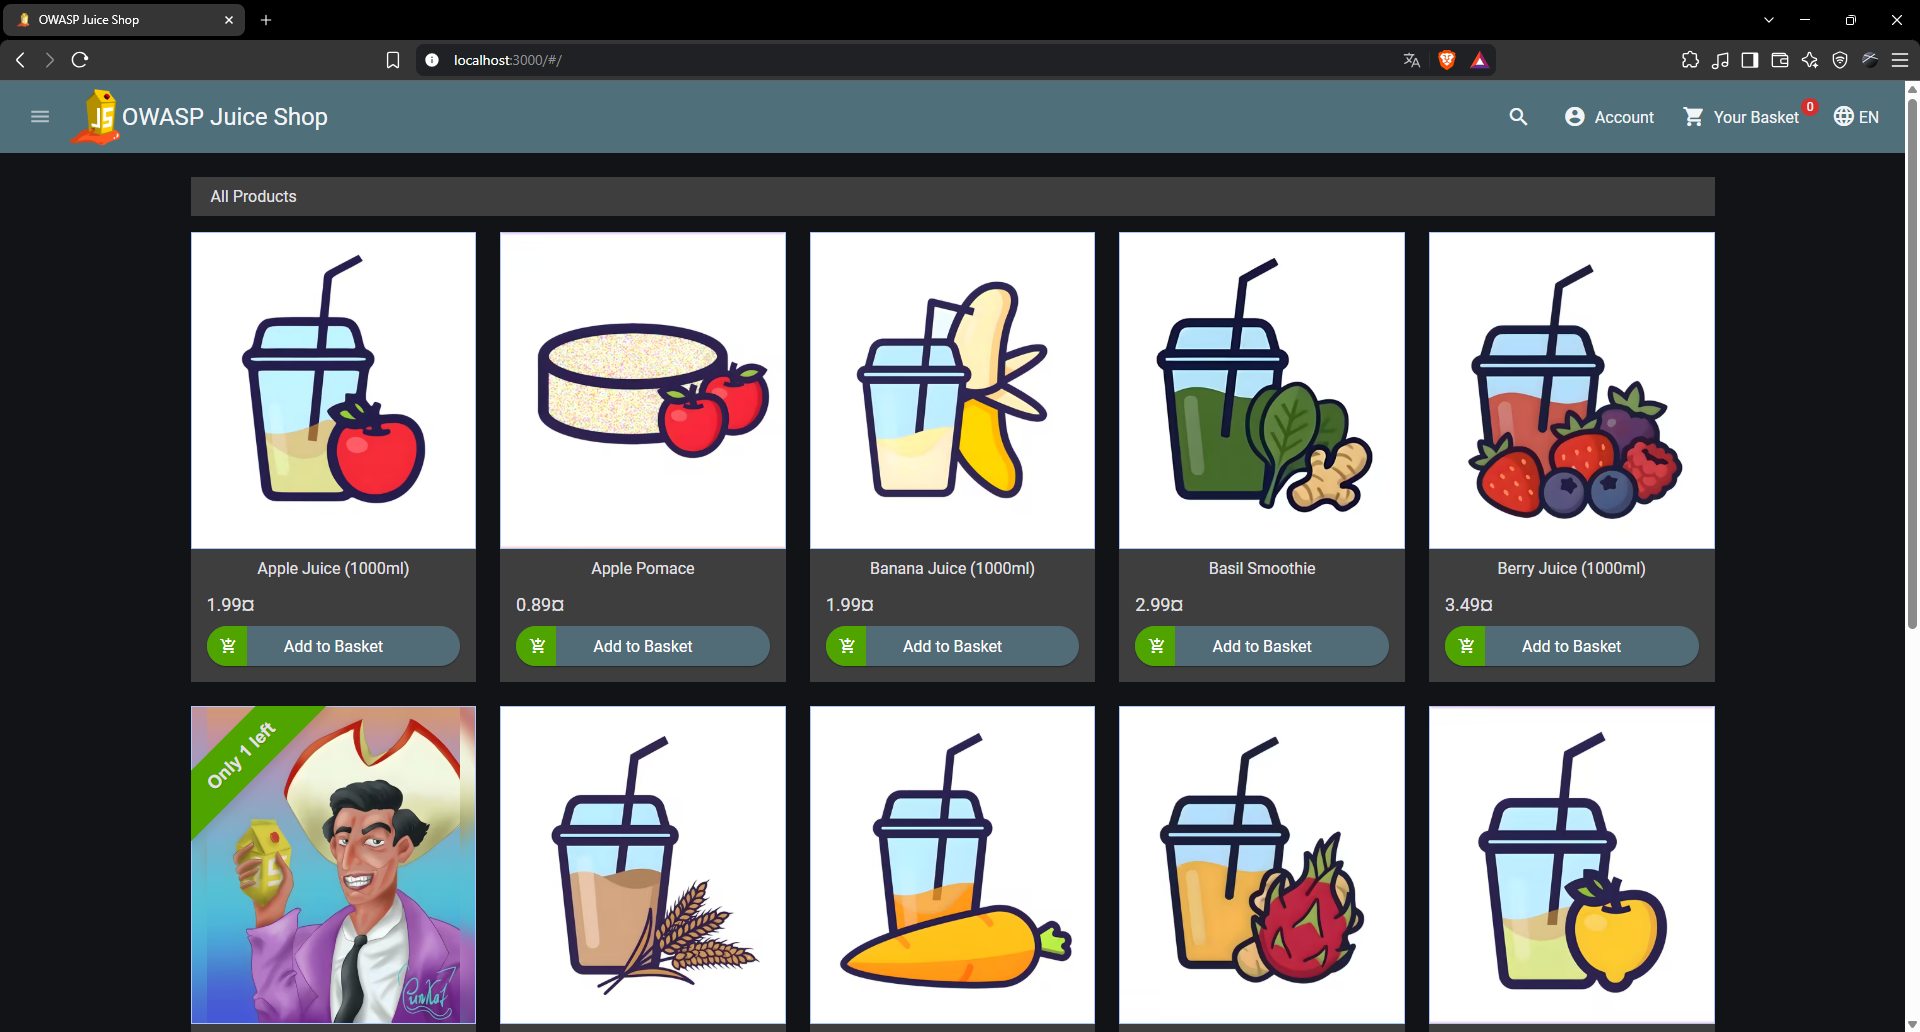
\includegraphics[width=0.85\textwidth]{01_acesso_juice-shop.png}
\caption{Acesso à OWASP Juice Shop}
\end{figure}

\paragraph{2. Score Board.}
O endereço \texttt{http://localhost:3000/\#/score-board} apresenta os desafios disponíveis e
confirma que a aplicação está configurada com os desafios inseguros.

\begin{figure}[H]
\centering
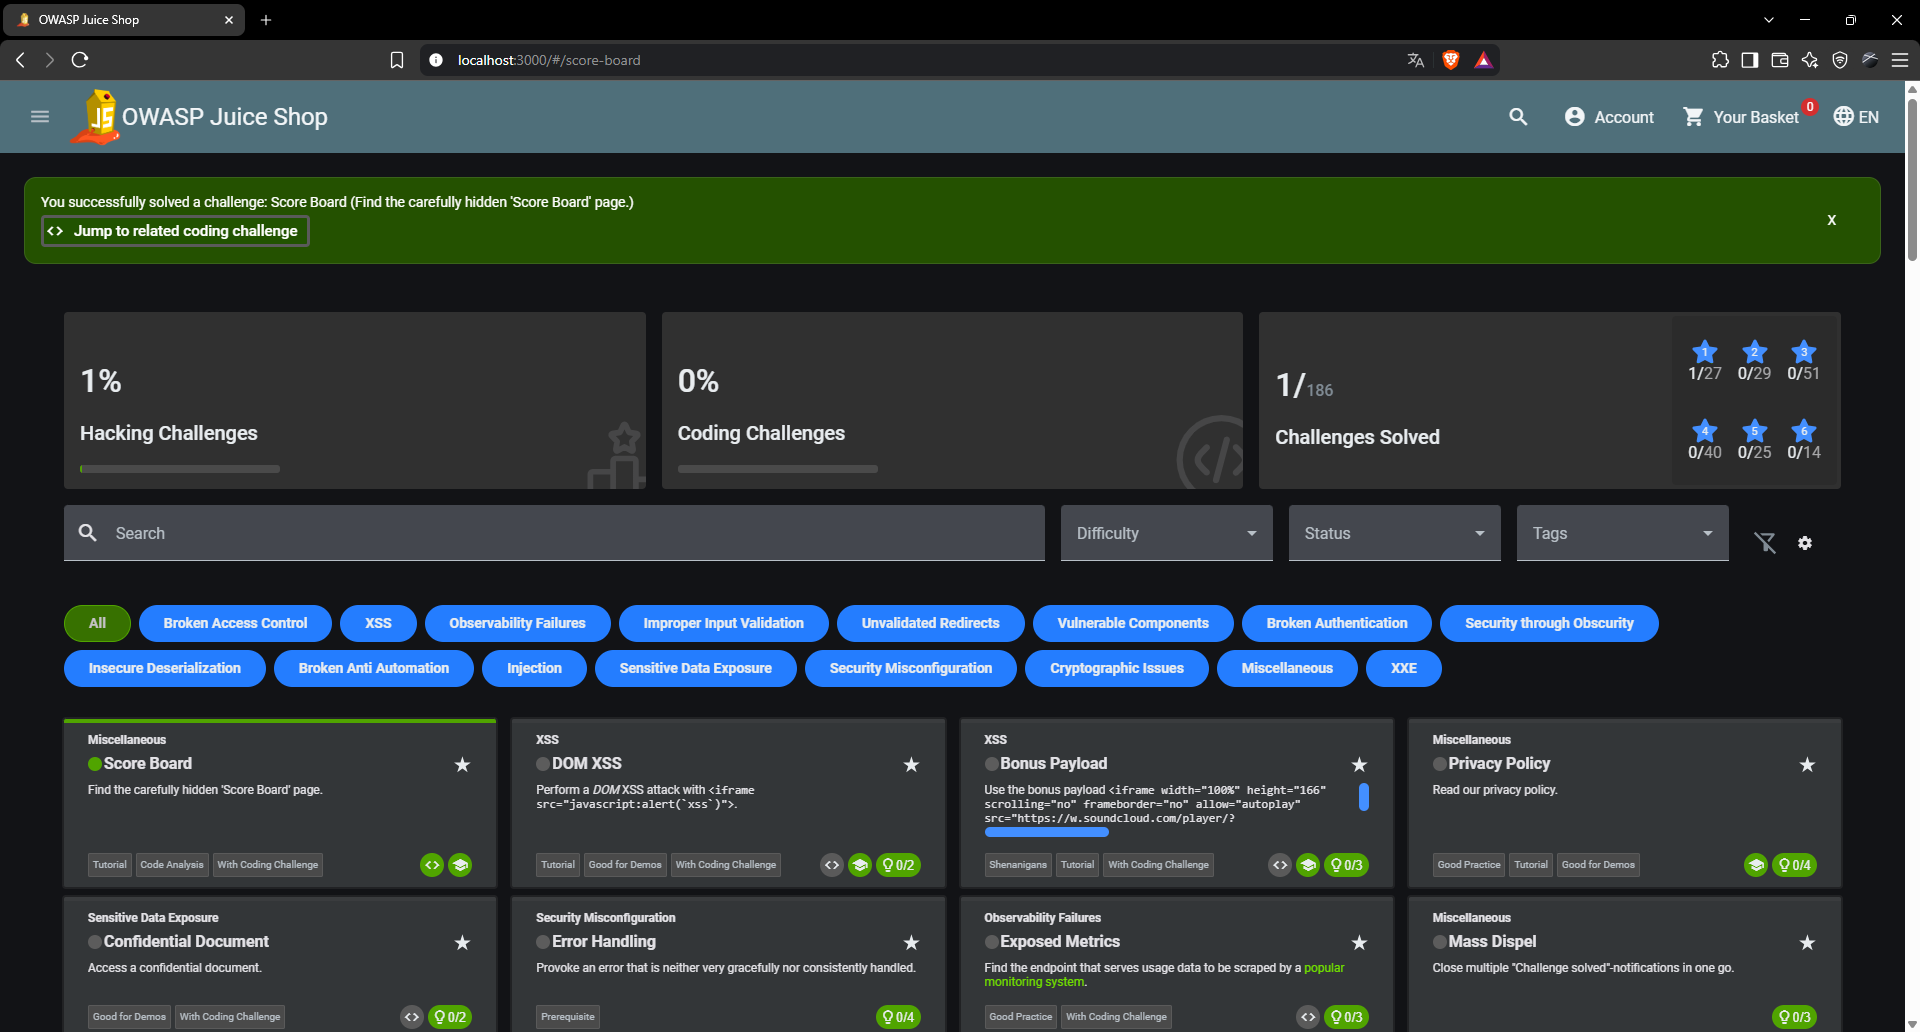
\includegraphics[width=0.85\textwidth]{02_acesso_score-board.png}
\caption{Score Board da Juice Shop}
\end{figure}

\paragraph{3. Configuração do ZAP.}
No ZAP foi usado \textbf{Manual Explore}, com o URL \texttt{http://localhost:3000}, e foi
iniciado o browser integrado. Desta forma, o tráfego do browser passou pelo proxy do ZAP. Depois
de abrir a aplicação, o site foi incluído no \textbf{Default Context} e o modo do ZAP foi
alterado para \textbf{Protected}.

\begin{figure}[H]
\centering
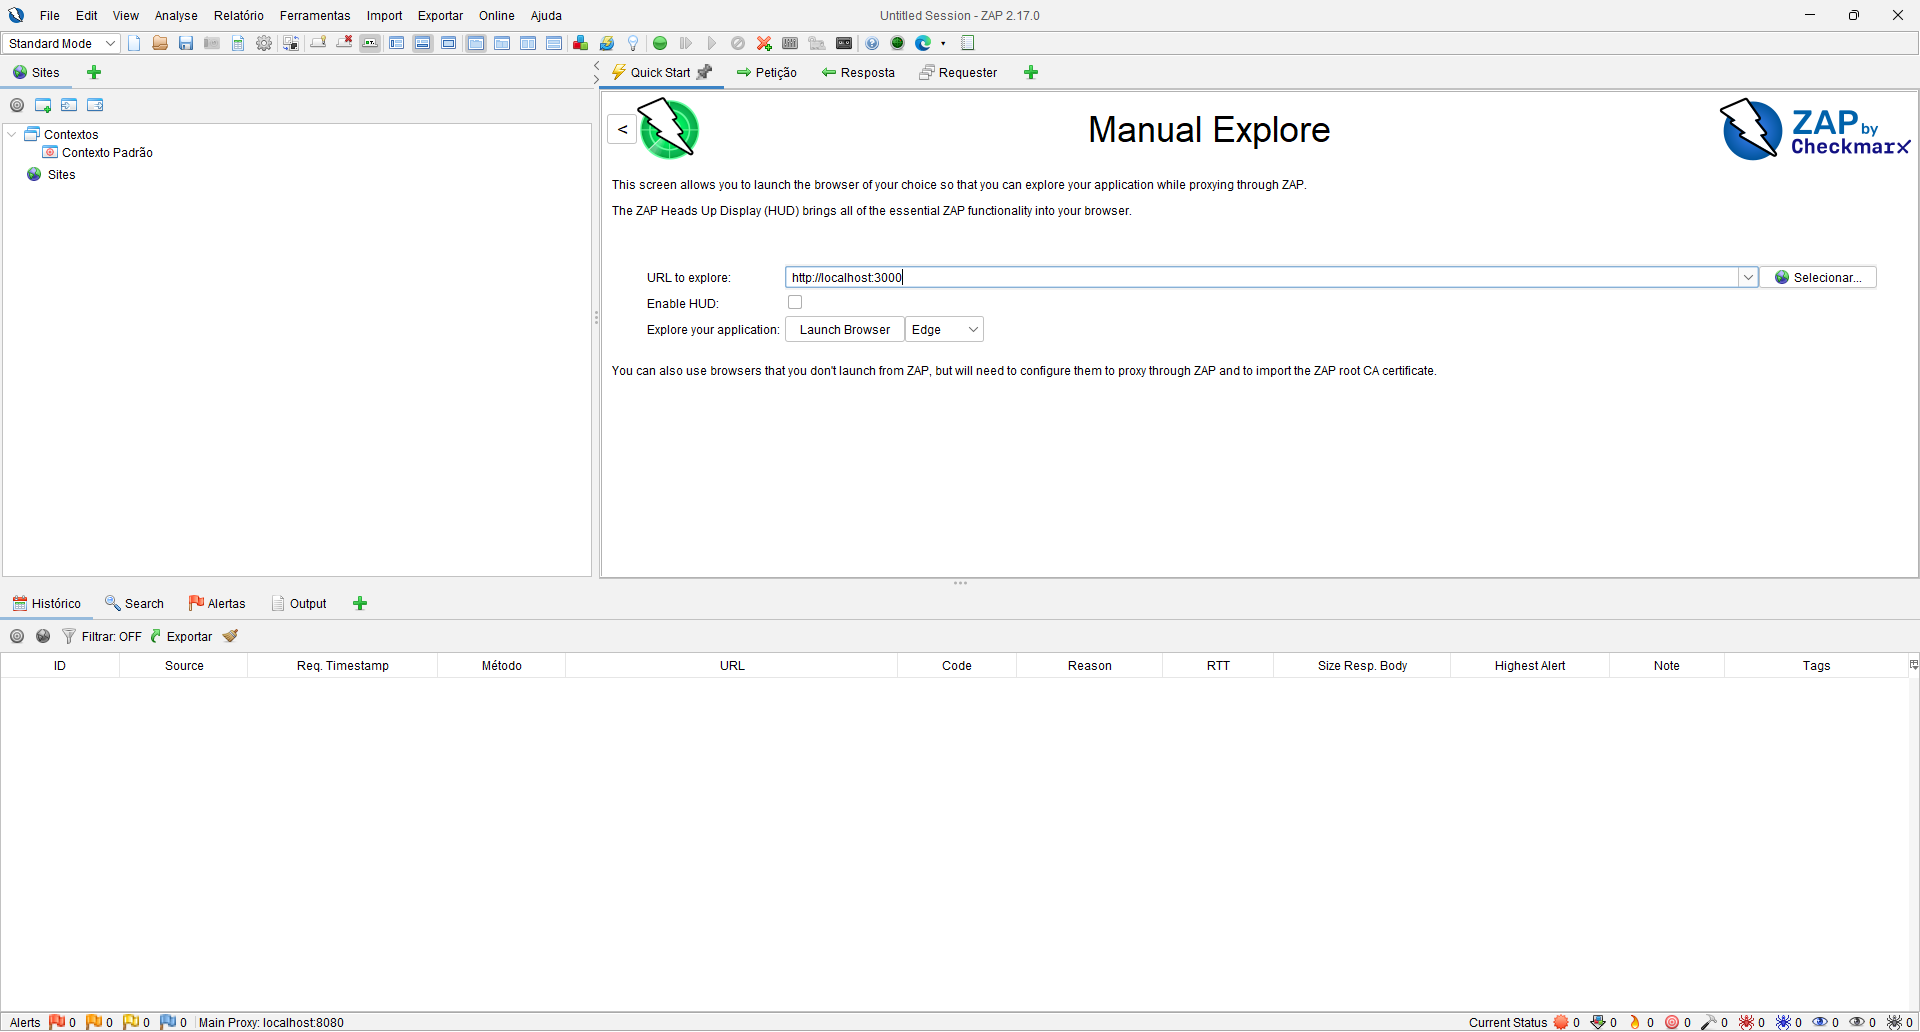
\includegraphics[width=0.85\textwidth]{03_start_zap.png}
\caption{Início do Manual Explore no ZAP}
\end{figure}

\begin{figure}[H]
\centering
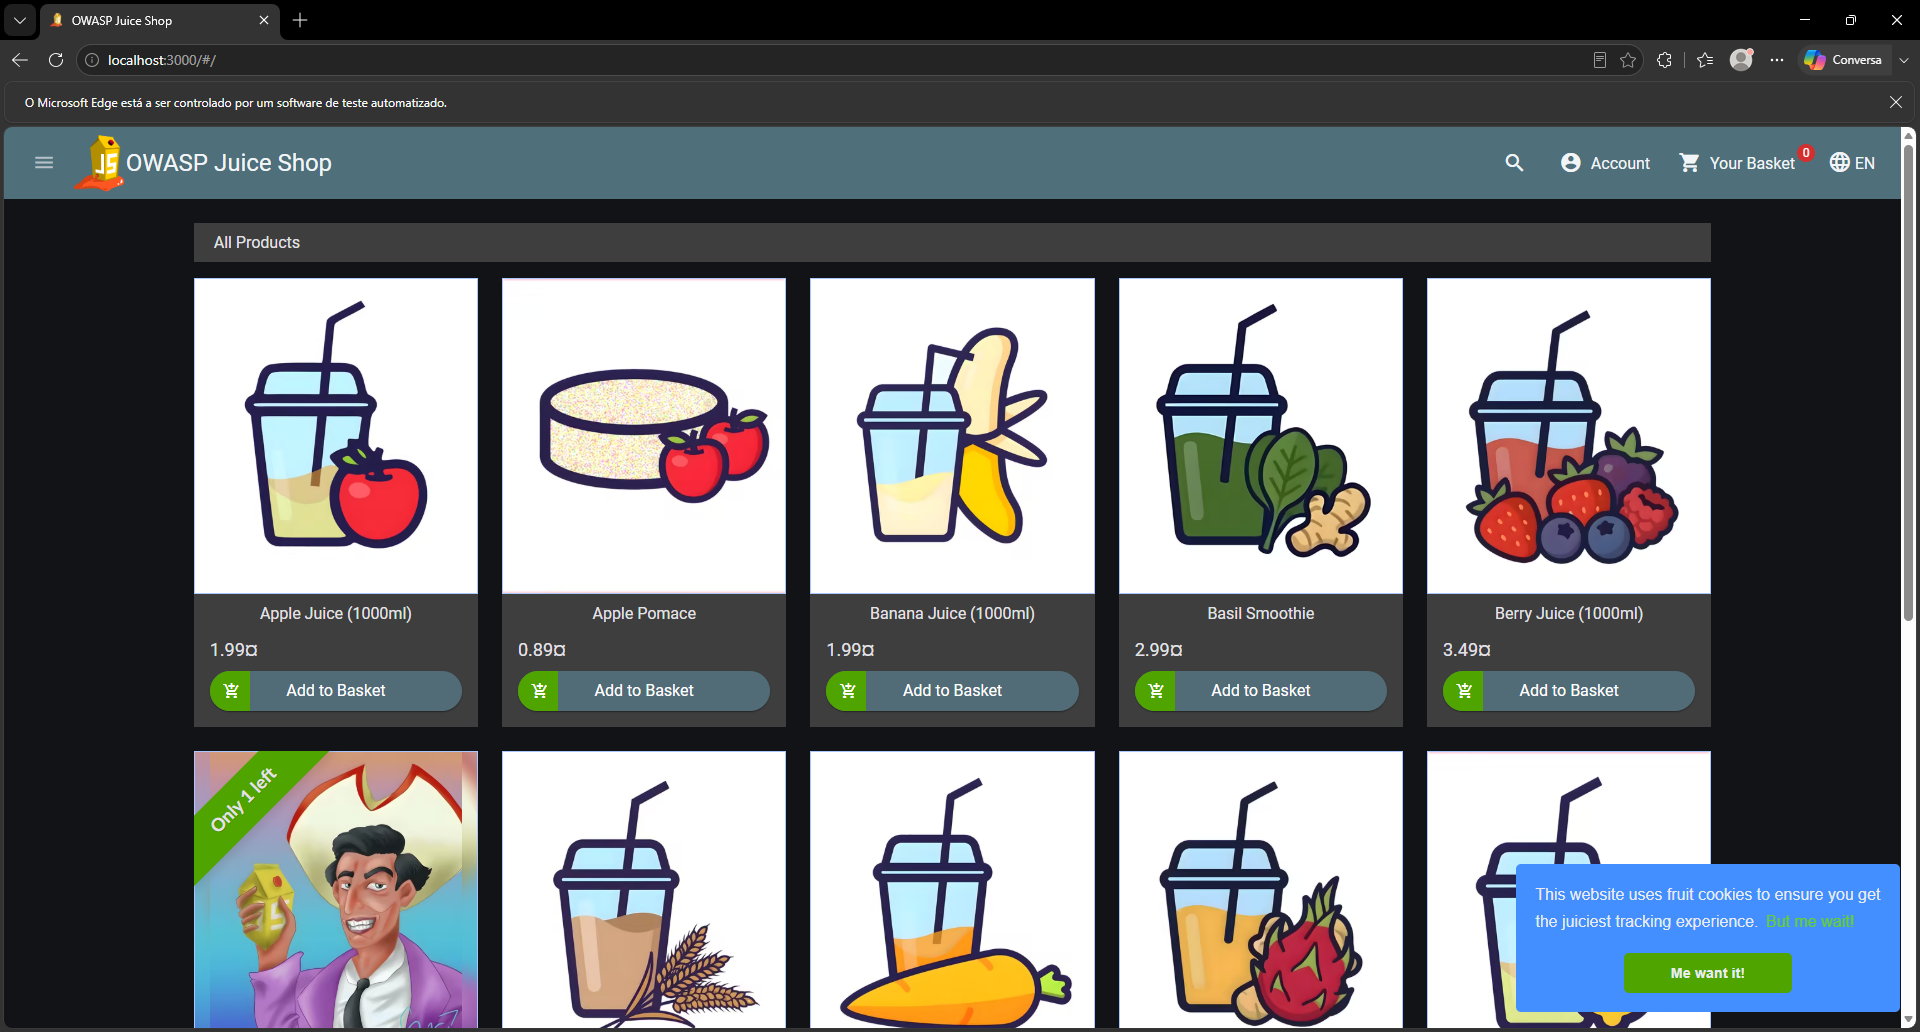
\includegraphics[width=0.85\textwidth]{04_open_zap_browser.png}
\caption{Aplicação aberta através do browser do ZAP}
\end{figure}

\subsection{B. Injeção de SQL no login}

\paragraph{5. Ataque de SQL injection.}
O formulário de login envia um pedido \texttt{POST} para \texttt{/rest/user/login}, com o corpo
JSON:
\begin{lstlisting}
{
  "email": "' or 1=1--",
  "password": "teste"
}
\end{lstlisting}
O valor inserido no campo \texttt{email} altera a consulta SQL. A expressão \texttt{1=1} é sempre
verdadeira e \texttt{--} comenta o restante da consulta, incluindo a verificação normal da
password. Assim, o primeiro registo compatível pode ser autenticado sem conhecer a password do
administrador.

\begin{figure}[H]
\centering
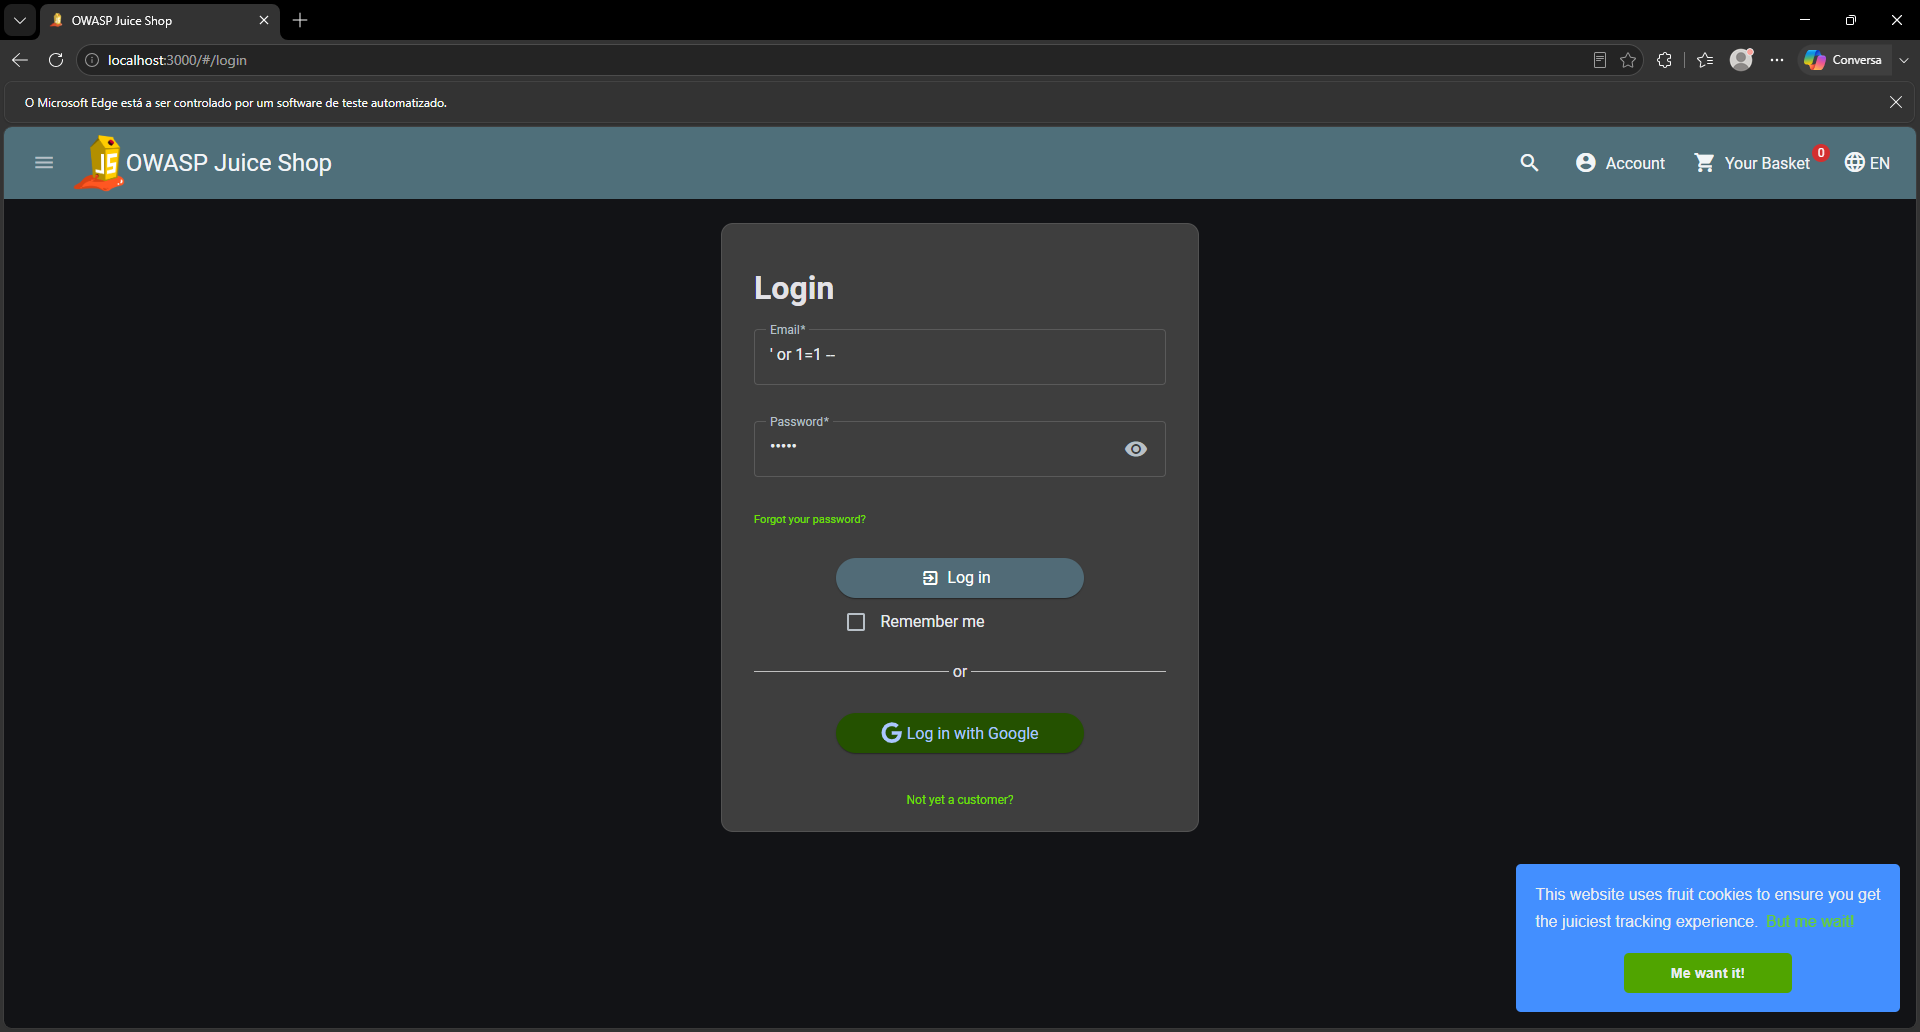
\includegraphics[width=0.85\textwidth]{05_inject_sql_login.png}
\caption{Payload de SQL injection no formulário de login}
\end{figure}

O resultado foi o acesso autenticado como \texttt{admin@juice-sh.op}, demonstrando que o desafio
\textbf{Login Admin} foi resolvido.

\begin{figure}[H]
\centering
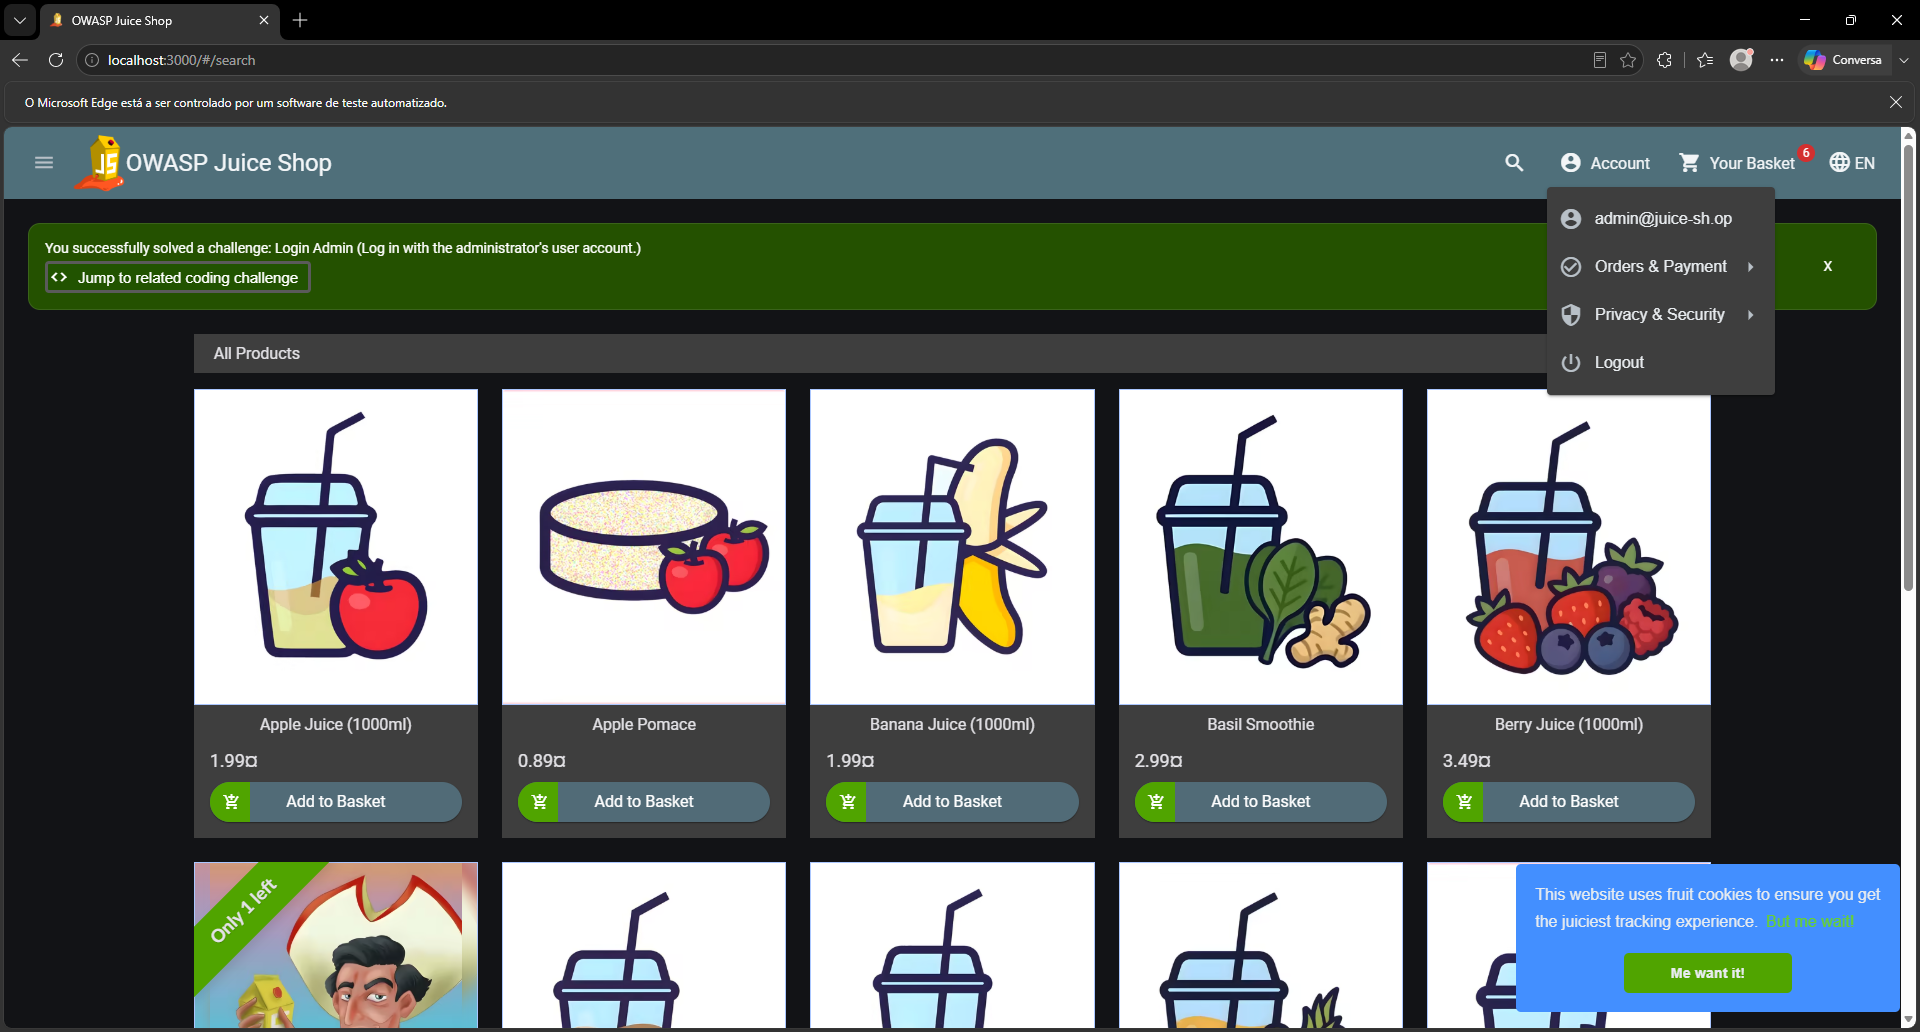
\includegraphics[width=0.85\textwidth]{05b_login_result.png}
\caption{Login efetuado como administrador}
\end{figure}

\paragraph{6. Pedido HTTP observado no ZAP.}
O pedido intercetado foi:
\begin{lstlisting}
POST http://localhost:3000/rest/user/login HTTP/1.1
Host: localhost:3000
Content-Type: application/json

{"email":"' or 1=1--","password":"teste"}
\end{lstlisting}
O ZAP registou a resposta com código \texttt{200 OK}, confirmando que a injeção foi aceite pelo
servidor.

\begin{figure}[H]
\centering
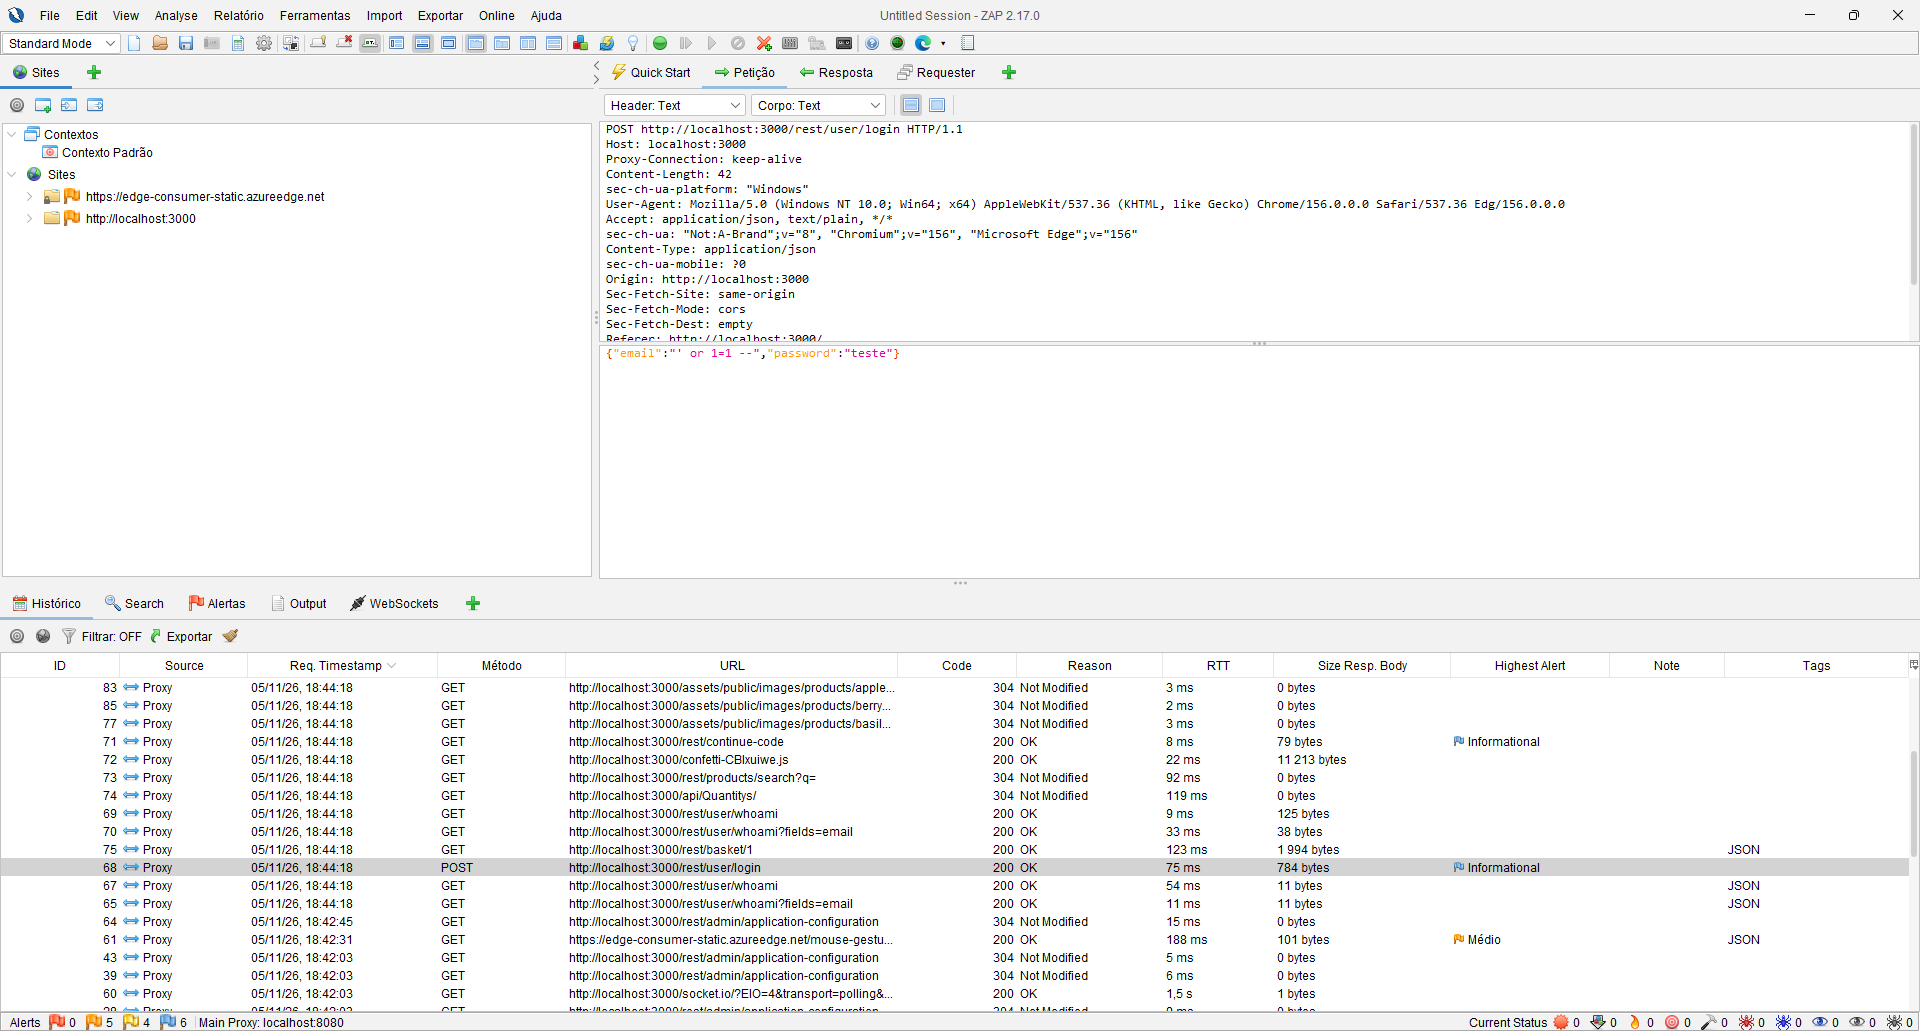
\includegraphics[width=0.85\textwidth]{06_zap_http_request_view.png}
\caption{Pedido HTTP observado no ZAP}
\end{figure}

\subsection{C. Fuzzing da senha do administrador}

\paragraph{7. Configuração e resultado do fuzzing.}
Foi capturado no ZAP um pedido de login válido para \texttt{admin@juice-sh.op}. No corpo do
pedido foi selecionado apenas o valor da password como posição de fuzzing:
\begin{lstlisting}[escapechar=!]
{"email":"admin@juice-sh.op","password":"admin!\S!000!\S!"}
\end{lstlisting}
No \textbf{Fuzzer} foi utilizada a lista \texttt{3-digits-000-999.txt}, acrescentada depois do
prefixo \texttt{admin}. Foram enviados 1000 pedidos, variando o sufixo entre \texttt{000} e
\texttt{999}. A maioria das respostas devolveu \texttt{401 Unauthorized}; a resposta diferente foi
a tentativa \texttt{admin123}, que devolveu \texttt{200 OK}.

\begin{figure}[H]
\centering
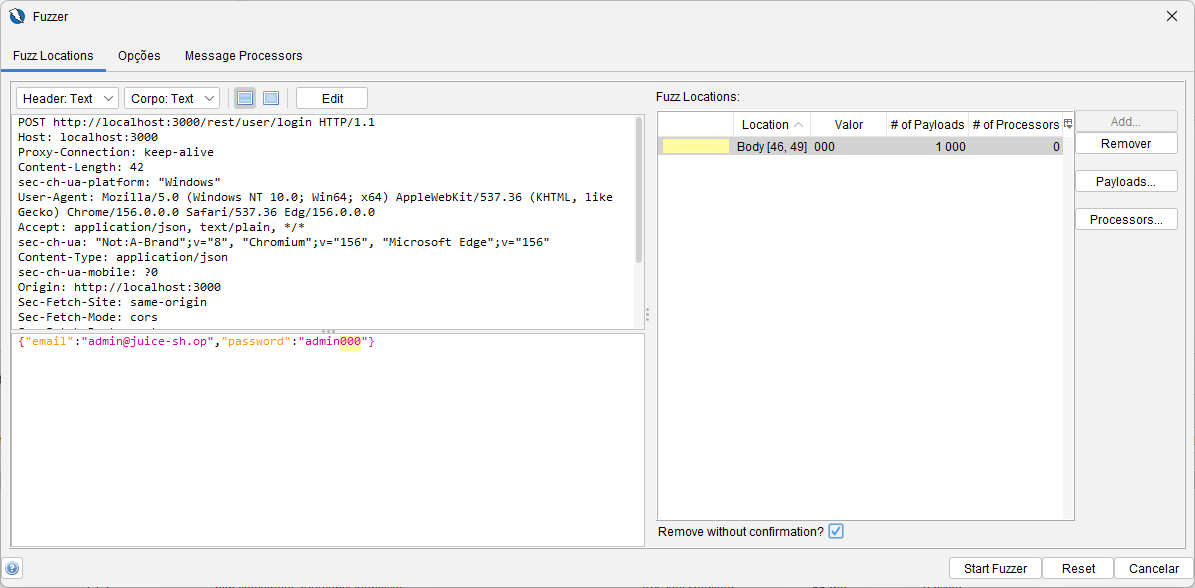
\includegraphics[width=0.85\textwidth]{07_set_fuzzer.png}
\caption{Pedido configurado no Fuzzer}
\end{figure}

\begin{figure}[H]
\centering
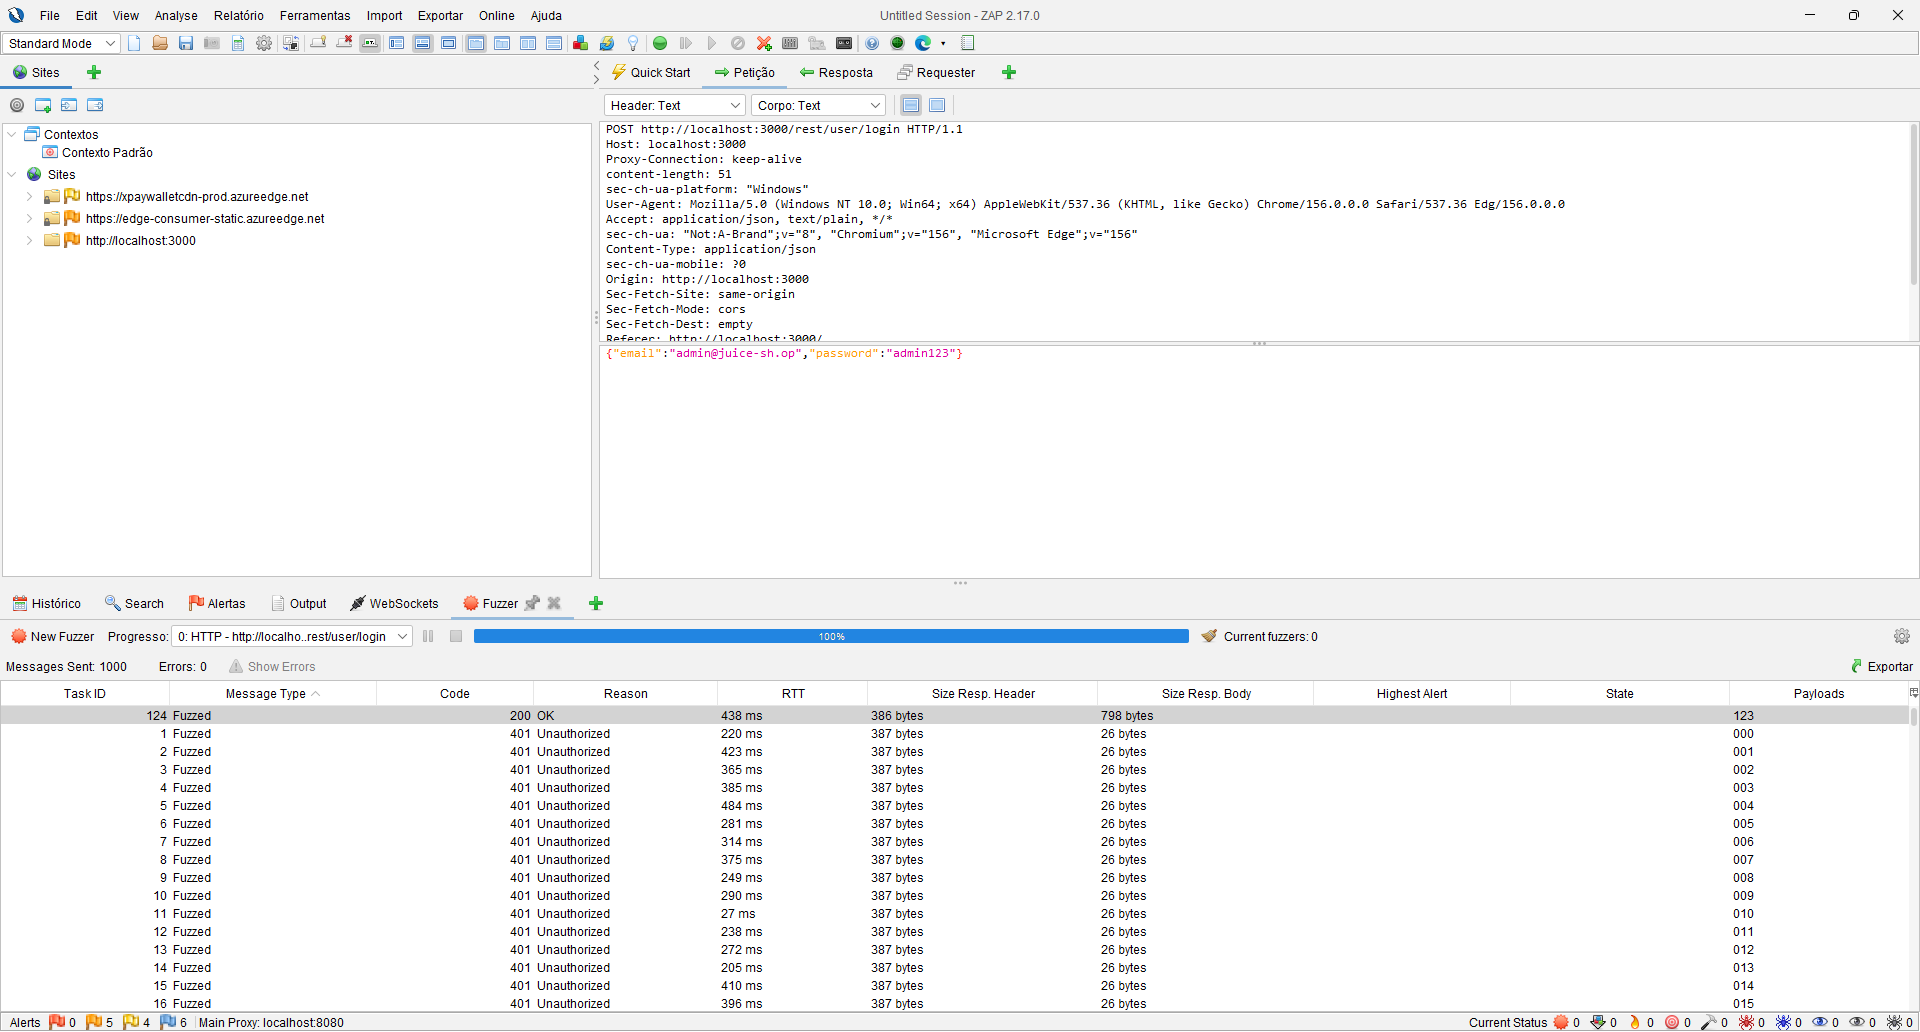
\includegraphics[width=0.85\textwidth]{07b_fuzzer_login_result.png}
\caption{Resultado das tentativas do Fuzzer}
\end{figure}

\begin{figure}[H]
\centering
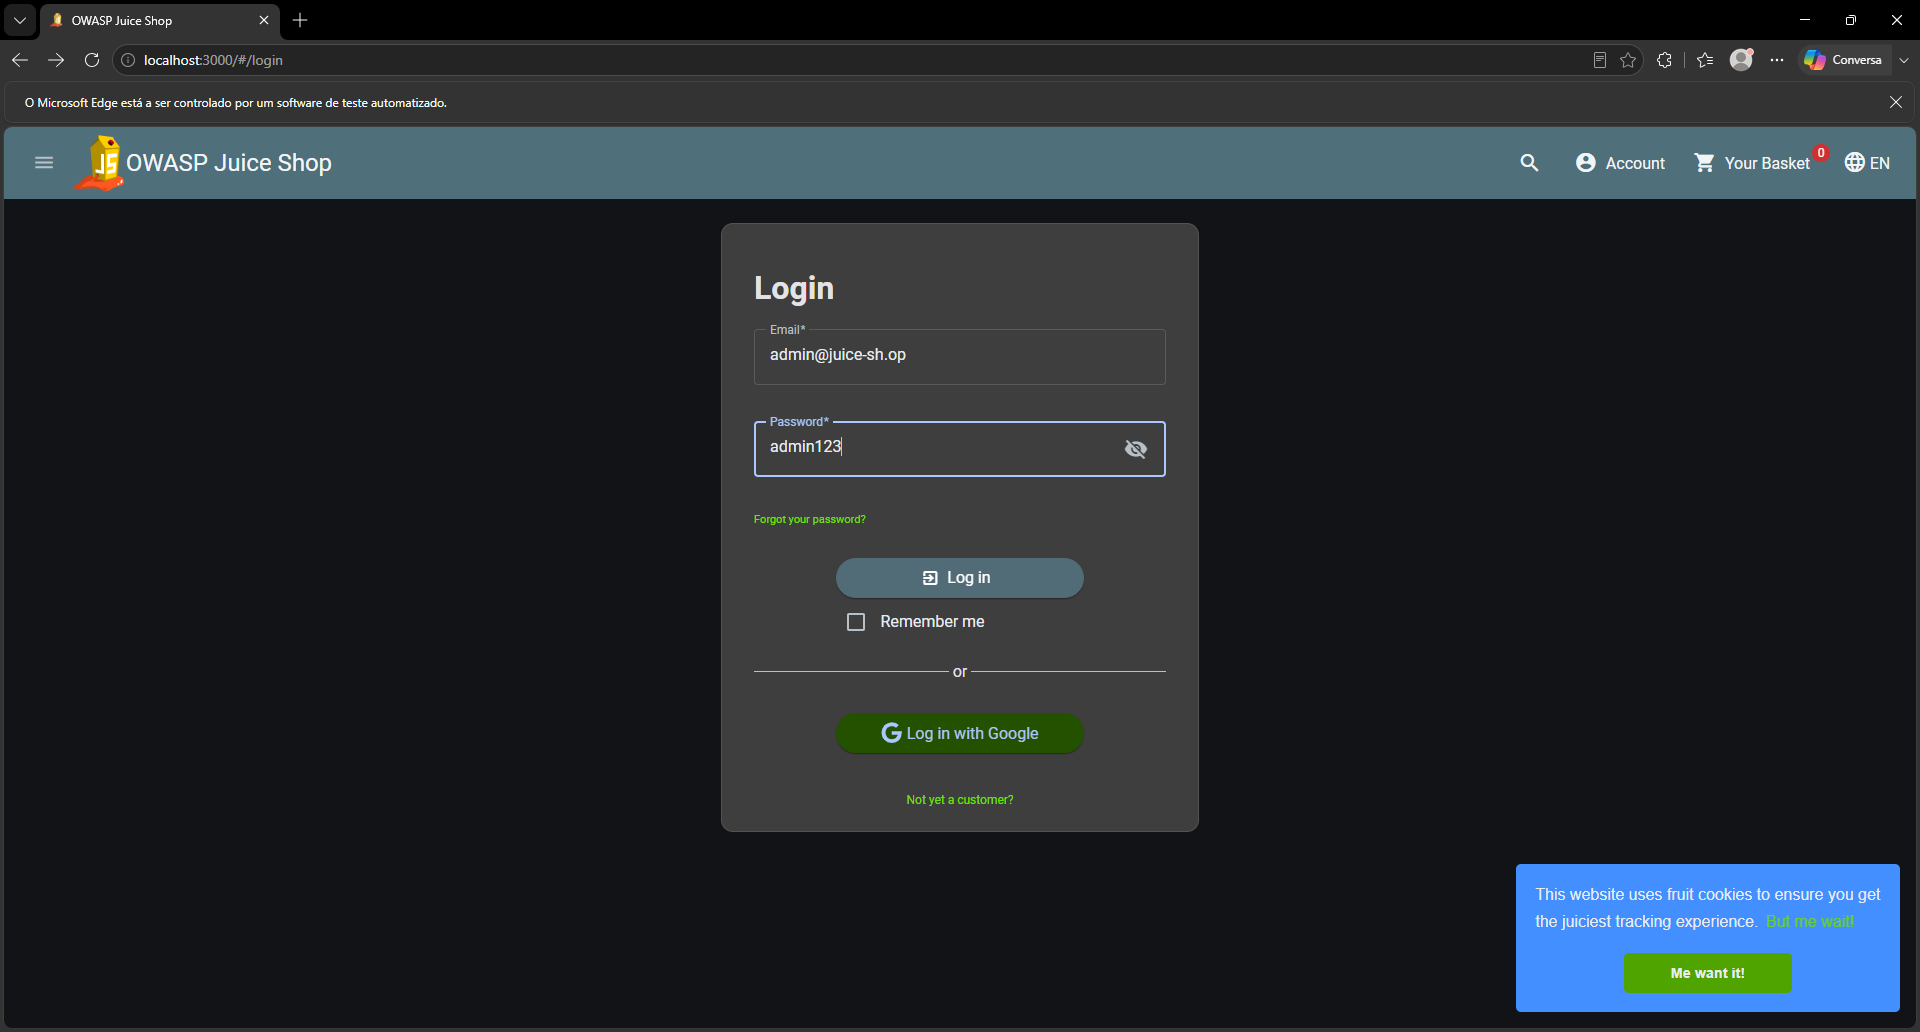
\includegraphics[width=0.85\textwidth]{07c_login_atempt.png}
\caption{Tentativa de login com \texttt{admin123}}
\end{figure}

\begin{figure}[H]
\centering
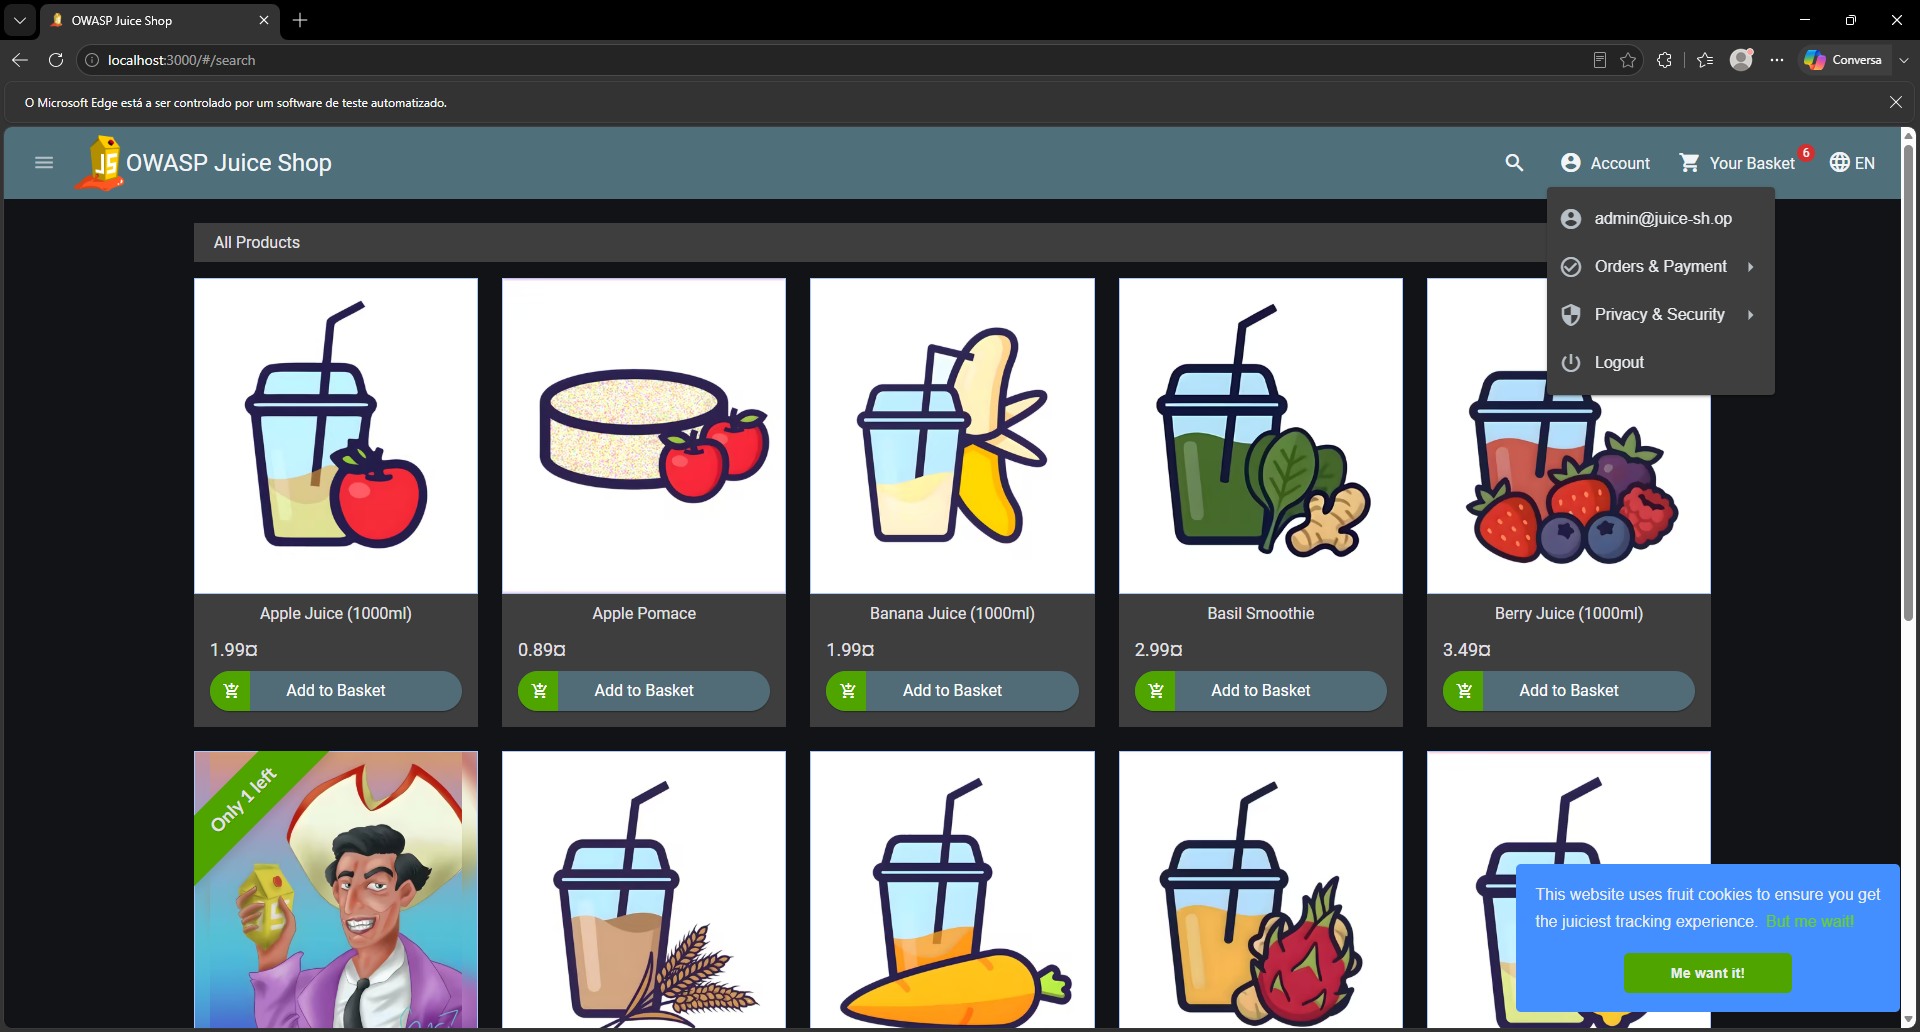
\includegraphics[width=0.85\textwidth]{07d_login_result.png}
\caption{Login bem-sucedido após o fuzzing}
\end{figure}

Assim, a password descoberta foi \texttt{admin123}.

\paragraph{8. Requisito ASVS violado.}
O comportamento viola o requisito \textbf{OWASP ASVS 5.0 --- V6.3.1}, que exige a implementação de
controlos contra ataques de \textit{credential stuffing} e \textit{password brute force}, de
acordo com a documentação de segurança da aplicação. Neste caso, o endpoint aceita 1000 tentativas
automatizadas sem limitação efetiva, atraso progressivo, bloqueio temporário ou outro mecanismo de
anti-automação. Um controlo adequado seria aplicar \textbf{rate limiting} por conta e por origem,
com atraso progressivo e, após várias falhas, um desafio adicional (por exemplo, CAPTCHA) ou
bloqueio temporário. O controlo não deve permitir que um atacante bloqueie permanentemente a conta
de uma vítima através de tentativas falsas.

\subsection{D. Broken Access Control}

\paragraph{9. Alteração de feedback (IDOR).}
A primeira imagem mostra a interceção do pedido para alterar o \texttt{id} do utilizador
(alterado para o \texttt{id} 1, que corresponde ao admin), tendo-se retirado o email de quem fez o
comentário, que aparecia no campo \texttt{comment}.

\begin{figure}[H]
\centering
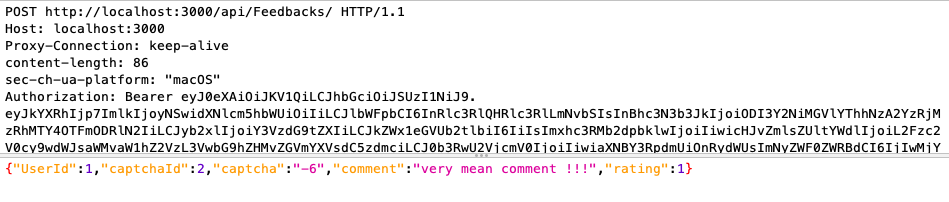
\includegraphics[width=0.85\textwidth]{09_change_feedback.png}
\caption{Interceção e alteração do pedido de feedback}
\end{figure}

A segunda imagem mostra o painel administrativo, onde é possível ver o feedback de todos os
utilizadores. O último feedback recebido está associado ao \texttt{userID} 1 e já aparece sem
email associado.

\begin{figure}[H]
\centering
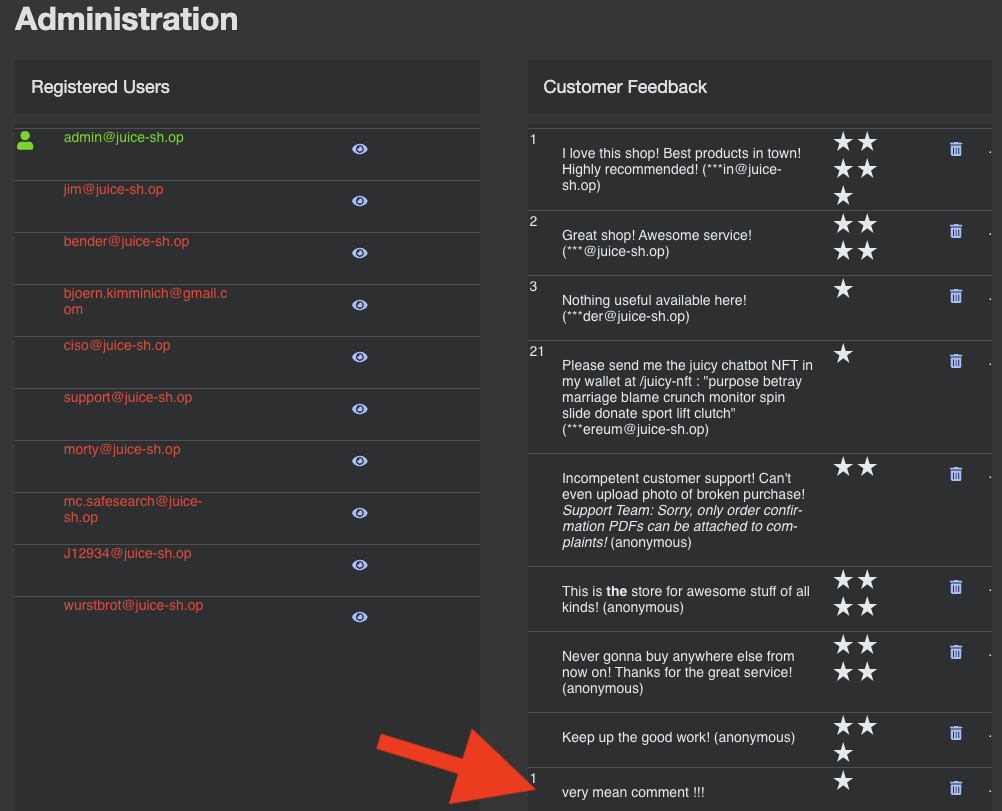
\includegraphics[width=0.85\textwidth]{09_administration_feedback_proof.png}
\caption{Painel administrativo com o feedback alterado (sem email, userID 1)}
\end{figure}

\paragraph{10. Ranking do IDOR/BOLA no OWASP Top 10:2025.}
Este tipo de vulnerabilidade enquadra-se na categoria \textbf{A01:2025 --- Broken Access Control},
que ocupa o 1.º lugar do OWASP Top 10:2025. Cobre explicitamente as falhas de autorização BOLA e
BFLA, que estão entre os padrões mais explorados em aplicações modernas orientadas a APIs. Em
comparação com 2021, surgiram novos métodos de ataque, tornando esta a categoria com o maior
número de CWEs mapeados.

\paragraph{11. CVE-2026-33760.}
O CVE-2026-33760 é uma vulnerabilidade de IDOR/BOLA no Langflow, uma ferramenta open-source para
construir e implementar agentes e workflows com IA, em que o \texttt{router/api/v1/monitor} expõe
7 endpoints que executam operações de leitura, escrita e eliminação sobre recursos pertencentes a
utilizadores sem fazer cumprir a verificação de propriedade. Na prática, permite que um utilizador
autenticado aceda, modifique ou elimine recursos de outros utilizadores sem autorização.

\subsection{E. Cross-Site Scripting (XSS)}

\paragraph{12. XSS refletido.}
Depois de iniciar sessão, foi aberta a funcionalidade de seguimento de encomendas. No
identificador da encomenda foi introduzido o payload:
\begin{lstlisting}
<iframe src="javascript:alert(`xss`)">
\end{lstlisting}
O valor foi refletido na página de resultados em \texttt{http://localhost:3000/\#/track-result}.
Como o conteúdo não foi corretamente codificado ou sanitizado antes de ser inserido no HTML, o
browser interpretou o payload como código HTML/JavaScript. Isto resolve o desafio \textbf{Reflect
XSS attack}.

% NOTA: a captura 12_find_vulnerable_page.png referida no enunciado nao foi encontrada
% na pasta TP_P3/images. Se existir, descomentar o bloco abaixo.
% \begin{figure}[H]
% \centering
% \includegraphics[width=0.85\textwidth]{12_find_vulnerable_page.png}
% \caption{Página vulnerável à injeção refletida}
% \end{figure}

\paragraph{13. XSS armazenado versus XSS refletido.}
\begin{itemize}
\item \textbf{XSS refletido:} o payload vem diretamente do pedido do atacante e é devolvido na
resposta da aplicação sem ser persistido. Normalmente é enviado através de um URL ou formulário
preparado pelo atacante, exigindo que a vítima aceda ao conteúdo malicioso.
\item \textbf{XSS armazenado:} o payload é guardado pelo servidor, por exemplo numa mensagem,
comentário ou perfil. É executado posteriormente sempre que uma vítima consulta a página que
apresenta esse conteúdo.
\end{itemize}
O XSS armazenado tende a ter maior alcance, porque não é necessário enviar um URL individual a
cada vítima.

\paragraph{14. Cookie \texttt{token} e payload JWT.}
Nas ferramentas de desenvolvimento do browser, o cookie \texttt{token} foi localizado nos cookies
da aplicação. O seu valor tem o formato \texttt{header.payload.signature}. Após copiar o token
para o \url{https://jwt.io}, a parte \textbf{Payload} pode ser decodificada como JSON. O
\textbf{Header} observado foi:
\begin{lstlisting}
{
  "typ": "JWT",
  "alg": "RS256"
}
\end{lstlisting}
O \textbf{Payload} observado foi:
\begin{lstlisting}
{
  "data": {
    "id": 1,
    "username": "",
    "email": "admin@juice-sh.op",
    "password": "0192023a7bbd73250516f069df18b500",
    "role": "admin",
    "deluxeToken": "",
    "lastLoginIp": "172.17.0.1",
    "profileImage": "assets/public/images/uploads/defaultAdmin.png",
    "totpSecret": "",
    "isActive": true,
    "createdAt": "2026-11-05 18:38:33.526 +00:00",
    "updatedAt": "2026-11-05 18:46:43.274 +00:00",
    "deletedAt": null
  },
  "bid": 1,
  "iat": 1793913831
}
\end{lstlisting}
O payload expõe informação sensível, incluindo o endereço de email, a função de administrador, o
endereço IP do último login e um valor associado à password. O campo \texttt{iat}
(\textit{issued at}) indica o instante de emissão do token. Não existe \texttt{exp} neste token,
pelo que o payload não define uma data de expiração. O payload é apenas codificado em Base64URL,
não cifrado; qualquer pessoa que obtenha o token consegue lê-lo. A assinatura RSA com
\texttt{RS256} permite ao servidor detetar alterações, mas não impede a leitura do conteúdo nem o
uso indevido de um token legítimo que tenha sido roubado.

\paragraph{15.a. Obtenção do cookie através de engenharia social.}
Um atacante poderia enviar à vítima uma mensagem convincente, por exemplo um suposto aviso de
encomenda contendo um link para a página vulnerável de seguimento. O link incluiria o payload XSS
e faria o browser executar JavaScript no contexto da Juice Shop. Esse script poderia ler
\texttt{document.cookie} se o cookie não tivesse a flag \texttt{HttpOnly} e enviar o valor do
cookie \texttt{token} para um servidor controlado pelo atacante. O atacante poderia então enviar
esse JWT nos pedidos seguintes e assumir a sessão da vítima, podendo consultar dados, alterar
informação e executar operações permitidas à conta, sem conhecer a password. As flags
\texttt{HttpOnly}, \texttt{Secure} e \texttt{SameSite} reduzem este risco, mas não substituem a
correção da vulnerabilidade XSS.

\paragraph{15.b. Avaliação do risco.}
Um vetor possível, usando fatores da metodologia OWASP Risk Rating, é:

\begin{center}
\begin{tabularx}{\textwidth}{@{}l l L@{}}
\toprule
\textbf{Fator} & \textbf{Avaliação} & \textbf{Justificação} \\
\midrule
Skill level & Baixo & O payload é curto e existem ferramentas públicas para o teste. \\
Motive & Alto & O roubo de sessão permite fraude e acesso a dados. \\
Opportunity & Média & A vítima tem de abrir o link preparado. \\
Size & Grande & Pode ser enviado a muitos utilizadores por engenharia social. \\
Ease of discovery & Fácil & A entrada é refletida na página de resultados. \\
Ease of exploit & Fácil & Basta preparar um URL com o payload. \\
Awareness & Média & A vulnerabilidade pode não ser evidente para o utilizador. \\
Intrusion detection & Baixa & Um pedido legítimo pode não parecer anómalo. \\
\bottomrule
\end{tabularx}
\end{center}

O impacto técnico é elevado: \textbf{confidencialidade alta} (acesso aos dados da conta),
\textbf{integridade alta} (ações em nome da vítima) e \textbf{disponibilidade baixa/média} (por
exemplo, alteração ou eliminação de dados). A combinação de exploração fácil, interação mínima e
possível comprometimento de sessões torna o risco global \textbf{alto}.

\end{document}
